% Options for packages loaded elsewhere
\PassOptionsToPackage{unicode}{hyperref}
\PassOptionsToPackage{hyphens}{url}
%
\documentclass[
]{article}
\usepackage{amsmath,amssymb}
\usepackage{iftex}
\ifPDFTeX
  \usepackage[T1]{fontenc}
  \usepackage[utf8]{inputenc}
  \usepackage{textcomp} % provide euro and other symbols
\else % if luatex or xetex
  \usepackage{unicode-math} % this also loads fontspec
  \defaultfontfeatures{Scale=MatchLowercase}
  \defaultfontfeatures[\rmfamily]{Ligatures=TeX,Scale=1}
\fi
\usepackage{lmodern}
\ifPDFTeX\else
  % xetex/luatex font selection
\fi
% Use upquote if available, for straight quotes in verbatim environments
\IfFileExists{upquote.sty}{\usepackage{upquote}}{}
\IfFileExists{microtype.sty}{% use microtype if available
  \usepackage[]{microtype}
  \UseMicrotypeSet[protrusion]{basicmath} % disable protrusion for tt fonts
}{}
\makeatletter
\@ifundefined{KOMAClassName}{% if non-KOMA class
  \IfFileExists{parskip.sty}{%
    \usepackage{parskip}
  }{% else
    \setlength{\parindent}{0pt}
    \setlength{\parskip}{6pt plus 2pt minus 1pt}}
}{% if KOMA class
  \KOMAoptions{parskip=half}}
\makeatother
\usepackage{xcolor}
\usepackage[margin=1in]{geometry}
\usepackage{color}
\usepackage{fancyvrb}
\newcommand{\VerbBar}{|}
\newcommand{\VERB}{\Verb[commandchars=\\\{\}]}
\DefineVerbatimEnvironment{Highlighting}{Verbatim}{commandchars=\\\{\}}
% Add ',fontsize=\small' for more characters per line
\usepackage{framed}
\definecolor{shadecolor}{RGB}{248,248,248}
\newenvironment{Shaded}{\begin{snugshade}}{\end{snugshade}}
\newcommand{\AlertTok}[1]{\textcolor[rgb]{0.94,0.16,0.16}{#1}}
\newcommand{\AnnotationTok}[1]{\textcolor[rgb]{0.56,0.35,0.01}{\textbf{\textit{#1}}}}
\newcommand{\AttributeTok}[1]{\textcolor[rgb]{0.13,0.29,0.53}{#1}}
\newcommand{\BaseNTok}[1]{\textcolor[rgb]{0.00,0.00,0.81}{#1}}
\newcommand{\BuiltInTok}[1]{#1}
\newcommand{\CharTok}[1]{\textcolor[rgb]{0.31,0.60,0.02}{#1}}
\newcommand{\CommentTok}[1]{\textcolor[rgb]{0.56,0.35,0.01}{\textit{#1}}}
\newcommand{\CommentVarTok}[1]{\textcolor[rgb]{0.56,0.35,0.01}{\textbf{\textit{#1}}}}
\newcommand{\ConstantTok}[1]{\textcolor[rgb]{0.56,0.35,0.01}{#1}}
\newcommand{\ControlFlowTok}[1]{\textcolor[rgb]{0.13,0.29,0.53}{\textbf{#1}}}
\newcommand{\DataTypeTok}[1]{\textcolor[rgb]{0.13,0.29,0.53}{#1}}
\newcommand{\DecValTok}[1]{\textcolor[rgb]{0.00,0.00,0.81}{#1}}
\newcommand{\DocumentationTok}[1]{\textcolor[rgb]{0.56,0.35,0.01}{\textbf{\textit{#1}}}}
\newcommand{\ErrorTok}[1]{\textcolor[rgb]{0.64,0.00,0.00}{\textbf{#1}}}
\newcommand{\ExtensionTok}[1]{#1}
\newcommand{\FloatTok}[1]{\textcolor[rgb]{0.00,0.00,0.81}{#1}}
\newcommand{\FunctionTok}[1]{\textcolor[rgb]{0.13,0.29,0.53}{\textbf{#1}}}
\newcommand{\ImportTok}[1]{#1}
\newcommand{\InformationTok}[1]{\textcolor[rgb]{0.56,0.35,0.01}{\textbf{\textit{#1}}}}
\newcommand{\KeywordTok}[1]{\textcolor[rgb]{0.13,0.29,0.53}{\textbf{#1}}}
\newcommand{\NormalTok}[1]{#1}
\newcommand{\OperatorTok}[1]{\textcolor[rgb]{0.81,0.36,0.00}{\textbf{#1}}}
\newcommand{\OtherTok}[1]{\textcolor[rgb]{0.56,0.35,0.01}{#1}}
\newcommand{\PreprocessorTok}[1]{\textcolor[rgb]{0.56,0.35,0.01}{\textit{#1}}}
\newcommand{\RegionMarkerTok}[1]{#1}
\newcommand{\SpecialCharTok}[1]{\textcolor[rgb]{0.81,0.36,0.00}{\textbf{#1}}}
\newcommand{\SpecialStringTok}[1]{\textcolor[rgb]{0.31,0.60,0.02}{#1}}
\newcommand{\StringTok}[1]{\textcolor[rgb]{0.31,0.60,0.02}{#1}}
\newcommand{\VariableTok}[1]{\textcolor[rgb]{0.00,0.00,0.00}{#1}}
\newcommand{\VerbatimStringTok}[1]{\textcolor[rgb]{0.31,0.60,0.02}{#1}}
\newcommand{\WarningTok}[1]{\textcolor[rgb]{0.56,0.35,0.01}{\textbf{\textit{#1}}}}
\usepackage{longtable,booktabs,array}
\usepackage{calc} % for calculating minipage widths
% Correct order of tables after \paragraph or \subparagraph
\usepackage{etoolbox}
\makeatletter
\patchcmd\longtable{\par}{\if@noskipsec\mbox{}\fi\par}{}{}
\makeatother
% Allow footnotes in longtable head/foot
\IfFileExists{footnotehyper.sty}{\usepackage{footnotehyper}}{\usepackage{footnote}}
\makesavenoteenv{longtable}
\usepackage{graphicx}
\makeatletter
\def\maxwidth{\ifdim\Gin@nat@width>\linewidth\linewidth\else\Gin@nat@width\fi}
\def\maxheight{\ifdim\Gin@nat@height>\textheight\textheight\else\Gin@nat@height\fi}
\makeatother
% Scale images if necessary, so that they will not overflow the page
% margins by default, and it is still possible to overwrite the defaults
% using explicit options in \includegraphics[width, height, ...]{}
\setkeys{Gin}{width=\maxwidth,height=\maxheight,keepaspectratio}
% Set default figure placement to htbp
\makeatletter
\def\fps@figure{htbp}
\makeatother
\setlength{\emergencystretch}{3em} % prevent overfull lines
\providecommand{\tightlist}{%
  \setlength{\itemsep}{0pt}\setlength{\parskip}{0pt}}
\setcounter{secnumdepth}{5}
\ifLuaTeX
  \usepackage{selnolig}  % disable illegal ligatures
\fi
\usepackage{bookmark}
\IfFileExists{xurl.sty}{\usepackage{xurl}}{} % add URL line breaks if available
\urlstyle{same}
\hypersetup{
  pdftitle={Statistical Learning Final Report},
  pdfauthor={Alberto Calabrese, Eleonora Mesaglio, Greta d'Amore Grelli},
  hidelinks,
  pdfcreator={LaTeX via pandoc}}

\title{Statistical Learning Final Report}
\author{Alberto Calabrese, Eleonora Mesaglio, Greta d'Amore Grelli}
\date{2024-06-09}

\begin{document}
\maketitle

{
\setcounter{tocdepth}{3}
\tableofcontents
}
\section{Introduction}\label{introduction}

Here Eleonora you can write the introduction of the project describing
the scope and the data used.

Thank you Albi, I will. What is our project scope though?

I think that we have to analyze the dataset and perform some statistical
analysis on it. We can start by calculating the correlation matrix and
then we can visualize the data through histograms, pairplots, barplots
and boxplots. Finally, we can perform a regression analysis.

\section{Data}\label{data}

The dataset we will analyze in this project is \emph{Starbucks Beverage
Components} from Kaggle, that you can find at the following link:
\url{https://www.kaggle.com/datasets/henryshan/starbucks}.

This data provides a comprehensive guide to the nutritional content of
the beverages available on the Starbucks menu. We have a total of
\(242\) samples described by \(18\) variables. These attributes include
the name of the beverage, its categorization and preparation method, the
total caloric content and the constituents of the beverage.

In the upcoming code lines, we import the dataset and generate a summary
visualization. This initial step allows us to gain a better
understanding of the data structure and the variables involved.

\begin{Shaded}
\begin{Highlighting}[]
\NormalTok{data }\OtherTok{\textless{}{-}} \FunctionTok{read.csv}\NormalTok{(}\StringTok{"Data/starbucks.csv"}\NormalTok{, }\AttributeTok{header =} \ConstantTok{TRUE}\NormalTok{, }\AttributeTok{sep =} \StringTok{","}\NormalTok{)}
\end{Highlighting}
\end{Shaded}

\subsection{Data Transformation}\label{data-transformation}

Note that several variables in our dataset, namely
``Vitamin.A\ldots.DV.'', ``Vitamin.C\ldots.DV.'', ``Calcium\ldots.DV.''
and ``Iron\ldots.DV.'', are represented as percentages. Consequently,
the percentage symbol is included in our data. However, when conducting
statistical analysis using R, the presence of non-numeric characters
such as the percentage symbol can cause complications, interfering with
the processing and analysis of the data. Therefore, we proceed to remove
it.

Similarly, as R primarily operates on numeric and categorical data, we
also convert all the other numerical variables into numeric format.

These preprocessing steps ensure a smooth and efficient analysis, making
it easier to explore, visualize, and understand our data.

\begin{Shaded}
\begin{Highlighting}[]
\CommentTok{\# Remove percentage sign from the data}
\NormalTok{data}\SpecialCharTok{$}\NormalTok{Vitamin.C....DV. }\OtherTok{\textless{}{-}} \FunctionTok{as.numeric}\NormalTok{(}\FunctionTok{gsub}\NormalTok{(}\StringTok{"\%"}\NormalTok{, }\StringTok{""}\NormalTok{, data}\SpecialCharTok{$}\NormalTok{Vitamin.C....DV.))}
\NormalTok{data}\SpecialCharTok{$}\NormalTok{Calcium....DV. }\OtherTok{\textless{}{-}} \FunctionTok{as.numeric}\NormalTok{(}\FunctionTok{gsub}\NormalTok{(}\StringTok{"\%"}\NormalTok{, }\StringTok{""}\NormalTok{, data}\SpecialCharTok{$}\NormalTok{Calcium....DV.))}
\NormalTok{data}\SpecialCharTok{$}\NormalTok{Iron....DV. }\OtherTok{\textless{}{-}} \FunctionTok{as.numeric}\NormalTok{(}\FunctionTok{gsub}\NormalTok{(}\StringTok{"\%"}\NormalTok{, }\StringTok{""}\NormalTok{, data}\SpecialCharTok{$}\NormalTok{Iron....DV.))}
\NormalTok{data}\SpecialCharTok{$}\NormalTok{Vitamin.A....DV. }\OtherTok{\textless{}{-}} \FunctionTok{as.numeric}\NormalTok{(}\FunctionTok{gsub}\NormalTok{(}\StringTok{"\%"}\NormalTok{, }\StringTok{""}\NormalTok{, data}\SpecialCharTok{$}\NormalTok{Vitamin.A....DV.))}
\CommentTok{\# Set the other variables as numeric}
\NormalTok{data}\SpecialCharTok{$}\NormalTok{Calories }\OtherTok{\textless{}{-}} \FunctionTok{as.numeric}\NormalTok{(data}\SpecialCharTok{$}\NormalTok{Calories)}
\NormalTok{data}\SpecialCharTok{$}\NormalTok{Trans.Fat..g. }\OtherTok{\textless{}{-}} \FunctionTok{as.numeric}\NormalTok{(data}\SpecialCharTok{$}\NormalTok{Trans.Fat..g.)}
\NormalTok{data}\SpecialCharTok{$}\NormalTok{Total.Fat..g. }\OtherTok{\textless{}{-}} \FunctionTok{as.numeric}\NormalTok{(data}\SpecialCharTok{$}\NormalTok{Total.Fat..g.)}
\NormalTok{data}\SpecialCharTok{$}\NormalTok{Cholesterol..mg. }\OtherTok{\textless{}{-}} \FunctionTok{as.numeric}\NormalTok{(data}\SpecialCharTok{$}\NormalTok{Cholesterol..mg.)}
\NormalTok{data}\SpecialCharTok{$}\NormalTok{Sodium..mg. }\OtherTok{\textless{}{-}} \FunctionTok{as.numeric}\NormalTok{(data}\SpecialCharTok{$}\NormalTok{Sodium..mg.)}
\NormalTok{data}\SpecialCharTok{$}\NormalTok{Total.Carbohydrates..g. }\OtherTok{\textless{}{-}} \FunctionTok{as.numeric}\NormalTok{(data}\SpecialCharTok{$}\NormalTok{Total.Carbohydrates..g.)}
\NormalTok{data}\SpecialCharTok{$}\NormalTok{Dietary.Fibre..g. }\OtherTok{\textless{}{-}} \FunctionTok{as.numeric}\NormalTok{(data}\SpecialCharTok{$}\NormalTok{Dietary.Fibre..g.)}
\NormalTok{data}\SpecialCharTok{$}\NormalTok{Sugars..g. }\OtherTok{\textless{}{-}} \FunctionTok{as.numeric}\NormalTok{(data}\SpecialCharTok{$}\NormalTok{Sugars..g.)}
\NormalTok{data}\SpecialCharTok{$}\NormalTok{Caffeine..mg. }\OtherTok{\textless{}{-}} \FunctionTok{as.numeric}\NormalTok{(data}\SpecialCharTok{$}\NormalTok{Caffeine..mg.)}
\end{Highlighting}
\end{Shaded}

\subsection{Data Cleaning}\label{data-cleaning}

Another challenge we have to face is the presence of missing data.
Indeed, in ``Caffeine..mg.'' column there are some NA values. This is a
common issue in data analysis and needs to be addressed appropriately to
ensure the validity of our statistical results.

One way to deal with these unwanted NA values is to omit the samples
containing them from our study. This guarantees that our analysis is
conducted solely on complete and dependable data. Alternatively, we can
fill them in with the average or the median of the observed values for
that specific attribute. This second method helps to preserve the
overall data distribution while addressing the missing data points.

In our work, we opt for the latter approach, replacing NA values with
the median. This choice is particularly suitable for our data, which is
skewed and contains outliers. Indeed, the median, being a measure of
central tendency that is not affected by extreme values, provides a more
robust replacement in the presence of outliers.

\begin{Shaded}
\begin{Highlighting}[]
\CommentTok{\# Summary of the Caffeine column}
\FunctionTok{summary}\NormalTok{(data}\SpecialCharTok{$}\NormalTok{Caffeine..mg.)}
\end{Highlighting}
\end{Shaded}

\begin{verbatim}
##    Min. 1st Qu.  Median    Mean 3rd Qu.    Max.    NA's 
##    0.00   50.00   75.00   89.52  142.50  410.00      23
\end{verbatim}

\begin{Shaded}
\begin{Highlighting}[]
\CommentTok{\# Replace NA values with the median}
\NormalTok{data\_cleaned }\OtherTok{\textless{}{-}}\NormalTok{ data}
\NormalTok{data\_cleaned}\SpecialCharTok{$}\NormalTok{Caffeine..mg.[}\FunctionTok{is.na}\NormalTok{(data\_cleaned}\SpecialCharTok{$}\NormalTok{Caffeine..mg.)] }\OtherTok{\textless{}{-}} \FunctionTok{median}\NormalTok{(}
\NormalTok{  data\_cleaned}\SpecialCharTok{$}\NormalTok{Caffeine..mg., }\AttributeTok{na.rm =} \ConstantTok{TRUE}\NormalTok{)}
\CommentTok{\# Summary of the Caffeine column after cleaning}
\FunctionTok{summary}\NormalTok{(data\_cleaned}\SpecialCharTok{$}\NormalTok{Caffeine..mg.)}
\end{Highlighting}
\end{Shaded}

\begin{verbatim}
##    Min. 1st Qu.  Median    Mean 3rd Qu.    Max. 
##    0.00   70.00   75.00   88.14  130.00  410.00
\end{verbatim}

\subsection{Rename Columns}\label{rename-columns}

Lastly, taking in consideration our cleaned data, we rename the columns
by removing dots and units of measure, in order to obtain a more
readable dataset.

\begin{Shaded}
\begin{Highlighting}[]
\FunctionTok{colnames}\NormalTok{(data\_cleaned) }\OtherTok{\textless{}{-}} \FunctionTok{c}\NormalTok{(}\StringTok{"Beverage\_category"}\NormalTok{, }\StringTok{"Beverage"}\NormalTok{, }\StringTok{"Beverage\_prep"}\NormalTok{,}
                            \StringTok{"Calories"}\NormalTok{, }\StringTok{"Total\_Fat"}\NormalTok{, }\StringTok{"Trans\_Fat"}\NormalTok{,}
                            \StringTok{"Saturated\_Fat"}\NormalTok{, }\StringTok{"Sodium"}\NormalTok{, }\StringTok{"Total\_Carbohydrates"}\NormalTok{,}
                            \StringTok{"Cholesterol"}\NormalTok{, }\StringTok{"Dietary\_Fibre"}\NormalTok{, }\StringTok{"Sugars"}\NormalTok{,}
                            \StringTok{"Protein"}\NormalTok{, }\StringTok{"Vitamin\_A"}\NormalTok{, }\StringTok{"Vitamin\_C"}\NormalTok{,}
                            \StringTok{"Calcium"}\NormalTok{, }\StringTok{"Iron"}\NormalTok{, }\StringTok{"Caffeine"}\NormalTok{)}
\end{Highlighting}
\end{Shaded}

\section{Correlation Analysis}\label{correlation-analysis}

After completing these preliminary preprocessing steps, we calculate the
correlation matrix for our dataset. This computation helps us in
comprehending the interrelationships among the dataset's variables. In
the correlation matrix, a value near to \(1\) at the \(ij\) position
indicates a strong positive correlation between the \(i\)-th and
\(j\)-th variables. Conversely, a value close to \(-1\) signifies a
strong negative correlation. A value near \(0\) suggests that the two
variables do not significantly influence each other.

Observe that the first three columns of our data are categorical
features, thus for these we cannot compute Pearson's correlation
coefficient. In the following code lines we remove them to compute and
plot such matrix.

\begin{Shaded}
\begin{Highlighting}[]
\CommentTok{\# Remove first 3 columns for the correlation matrix since them are categorical}
\NormalTok{data\_num }\OtherTok{\textless{}{-}}\NormalTok{ data\_cleaned[, }\FunctionTok{sapply}\NormalTok{(data\_cleaned, is.numeric)]}
\NormalTok{correlation\_matrix }\OtherTok{\textless{}{-}} \FunctionTok{cor}\NormalTok{(data\_num)}
\CommentTok{\# Plot the correlation matrix using corrplot}
\FunctionTok{corrplot}\NormalTok{(correlation\_matrix, }\AttributeTok{method =} \StringTok{"number"}\NormalTok{, }\AttributeTok{tl.col =} \StringTok{"black"}\NormalTok{, }
         \AttributeTok{tl.srt =} \DecValTok{45}\NormalTok{, }\AttributeTok{addCoef.col =} \StringTok{"black"}\NormalTok{, }\AttributeTok{number.cex =} \FloatTok{0.5}\NormalTok{, }\AttributeTok{tl.cex =} \FloatTok{0.7}\NormalTok{)}
\end{Highlighting}
\end{Shaded}

\begin{center}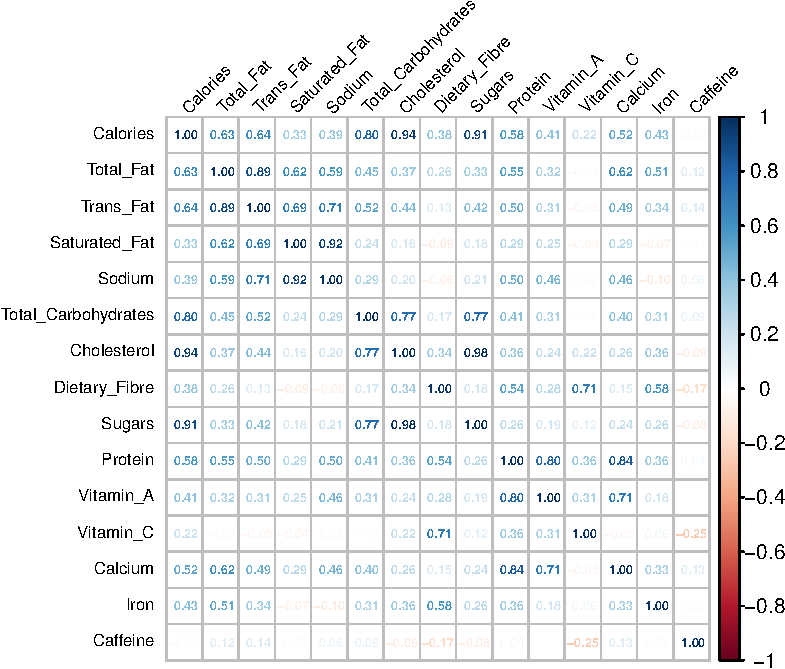
\includegraphics{Statistical_Learning_Final_Report_files/figure-latex/correlation_analysis-1} \end{center}

\section{Data Visualization}\label{data-visualization}

Data visualization is a powerful tool that allows us to uncover
patterns, correlations and outliers in our data. It provides visual
information on the dataset in our analysis, representing large amounts
of data in a clear and comprehensive way and underlining the
relationships among them. This enables us to recognize patterns quickly.

So, let us transform our raw data into graphical representations, to
gain a more comprehensive understanding of the information at hand.

\subsection{Histograms}\label{histograms}

Histograms serve as a graphical interpretation of data distribution. In
a histogram, each bar corresponds to the counted frequency within each
bin or interval. We introduce these plots to see if our data is normally
distributed, skewed, or has outlier values.

\begin{Shaded}
\begin{Highlighting}[]
\CommentTok{\# Histogram of the data with density distribution}
\FunctionTok{par}\NormalTok{(}\AttributeTok{mfrow =} \FunctionTok{c}\NormalTok{(}\DecValTok{5}\NormalTok{, }\DecValTok{3}\NormalTok{), }\AttributeTok{mar =} \FunctionTok{c}\NormalTok{(}\DecValTok{2}\NormalTok{, }\DecValTok{2}\NormalTok{, }\DecValTok{2}\NormalTok{, }\DecValTok{2}\NormalTok{))}
\NormalTok{col }\OtherTok{\textless{}{-}} \FunctionTok{c}\NormalTok{(}\StringTok{\textquotesingle{}\#ff0000\textquotesingle{}}\NormalTok{, }\StringTok{\textquotesingle{}\#f70028\textquotesingle{}}\NormalTok{, }\StringTok{\textquotesingle{}\#ee0040\textquotesingle{}}\NormalTok{, }\StringTok{\textquotesingle{}\#e50055\textquotesingle{}}\NormalTok{, }\StringTok{\textquotesingle{}\#dc0069\textquotesingle{}}\NormalTok{,}
         \StringTok{\textquotesingle{}\#d2007b\textquotesingle{}}\NormalTok{, }\StringTok{\textquotesingle{}\#c7008d\textquotesingle{}}\NormalTok{, }\StringTok{\textquotesingle{}\#bb009e\textquotesingle{}}\NormalTok{, }\StringTok{\textquotesingle{}\#ae00ae\textquotesingle{}}\NormalTok{, }\StringTok{\textquotesingle{}\#a000be\textquotesingle{}}\NormalTok{,}
         \StringTok{\textquotesingle{}\#8f00cc\textquotesingle{}}\NormalTok{, }\StringTok{\textquotesingle{}\#7d00da\textquotesingle{}}\NormalTok{, }\StringTok{\textquotesingle{}\#6700e7\textquotesingle{}}\NormalTok{, }\StringTok{\textquotesingle{}\#4900f3\textquotesingle{}}\NormalTok{, }\StringTok{\textquotesingle{}\#0000ff\textquotesingle{}}\NormalTok{)}
\ControlFlowTok{for}\NormalTok{ (i }\ControlFlowTok{in} \DecValTok{1}\SpecialCharTok{:}\FunctionTok{ncol}\NormalTok{(data\_num)) \{}
  \FunctionTok{hist}\NormalTok{(data\_num[, i], }\AttributeTok{main =} \FunctionTok{colnames}\NormalTok{(data\_num)[i],}
       \AttributeTok{xlab =} \FunctionTok{colnames}\NormalTok{(data\_num)[i], }\AttributeTok{col =}\NormalTok{ col[i], }\AttributeTok{freq =} \ConstantTok{FALSE}\NormalTok{)}
\NormalTok{  dens }\OtherTok{\textless{}{-}} \FunctionTok{density}\NormalTok{(data\_num[, i], }\AttributeTok{na.rm=}\ConstantTok{TRUE}\NormalTok{, }\AttributeTok{adjust=}\FloatTok{1.25}\NormalTok{)}
  \FunctionTok{lines}\NormalTok{(dens, }\AttributeTok{col =} \StringTok{"black"}\NormalTok{, }\AttributeTok{lwd =} \DecValTok{2}\NormalTok{)}
\NormalTok{\}}
\end{Highlighting}
\end{Shaded}

\begin{center}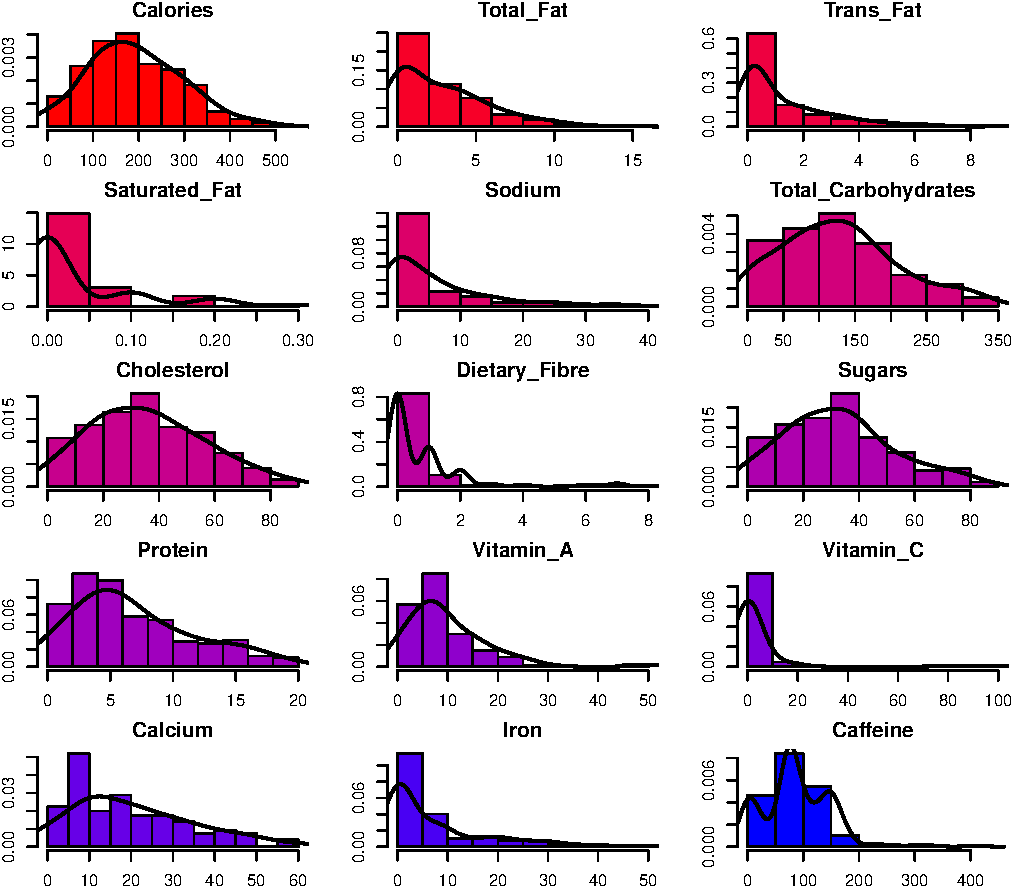
\includegraphics{Statistical_Learning_Final_Report_files/figure-latex/histograms-1} \end{center}

By looking at the graphs, we can notice that the variables ``Calories'',
``Total\_Carbohydrates'', ``Cholesterol'', and ``Sugars'' exhibit
distributions that are nearly normal. Conversely, the distributions of
the remaining variables display a noticeable skewness towards the left.

\subsection{Pairplot}\label{pairplot}

\textbf{io questi li toglierei. tanto spazio}

We will plot a pairplot to visualize the relationship between the
variables. The pairplot is a grid of scatterplots that shows the
relationship between each pair of variables in the dataset. This
visualization helps us to identify patterns and correlations between the
variables.

First of all we have to define the function for the pairplot. We will
define a function for the histogram, the correlation and the smooth
line.

Then we create the pairplot using the defined functions.

\begin{Shaded}
\begin{Highlighting}[]
\FunctionTok{pairs}\NormalTok{(data\_num, }
      \AttributeTok{diag.panel =}\NormalTok{ panel.hist,}
      \AttributeTok{upper.panel =}\NormalTok{ panel.cor, }
      \AttributeTok{lower.panel =}\NormalTok{ panel.smooth,}
      \AttributeTok{colour =} \StringTok{"\#4ea5ff"}\NormalTok{)}
\end{Highlighting}
\end{Shaded}

\begin{center}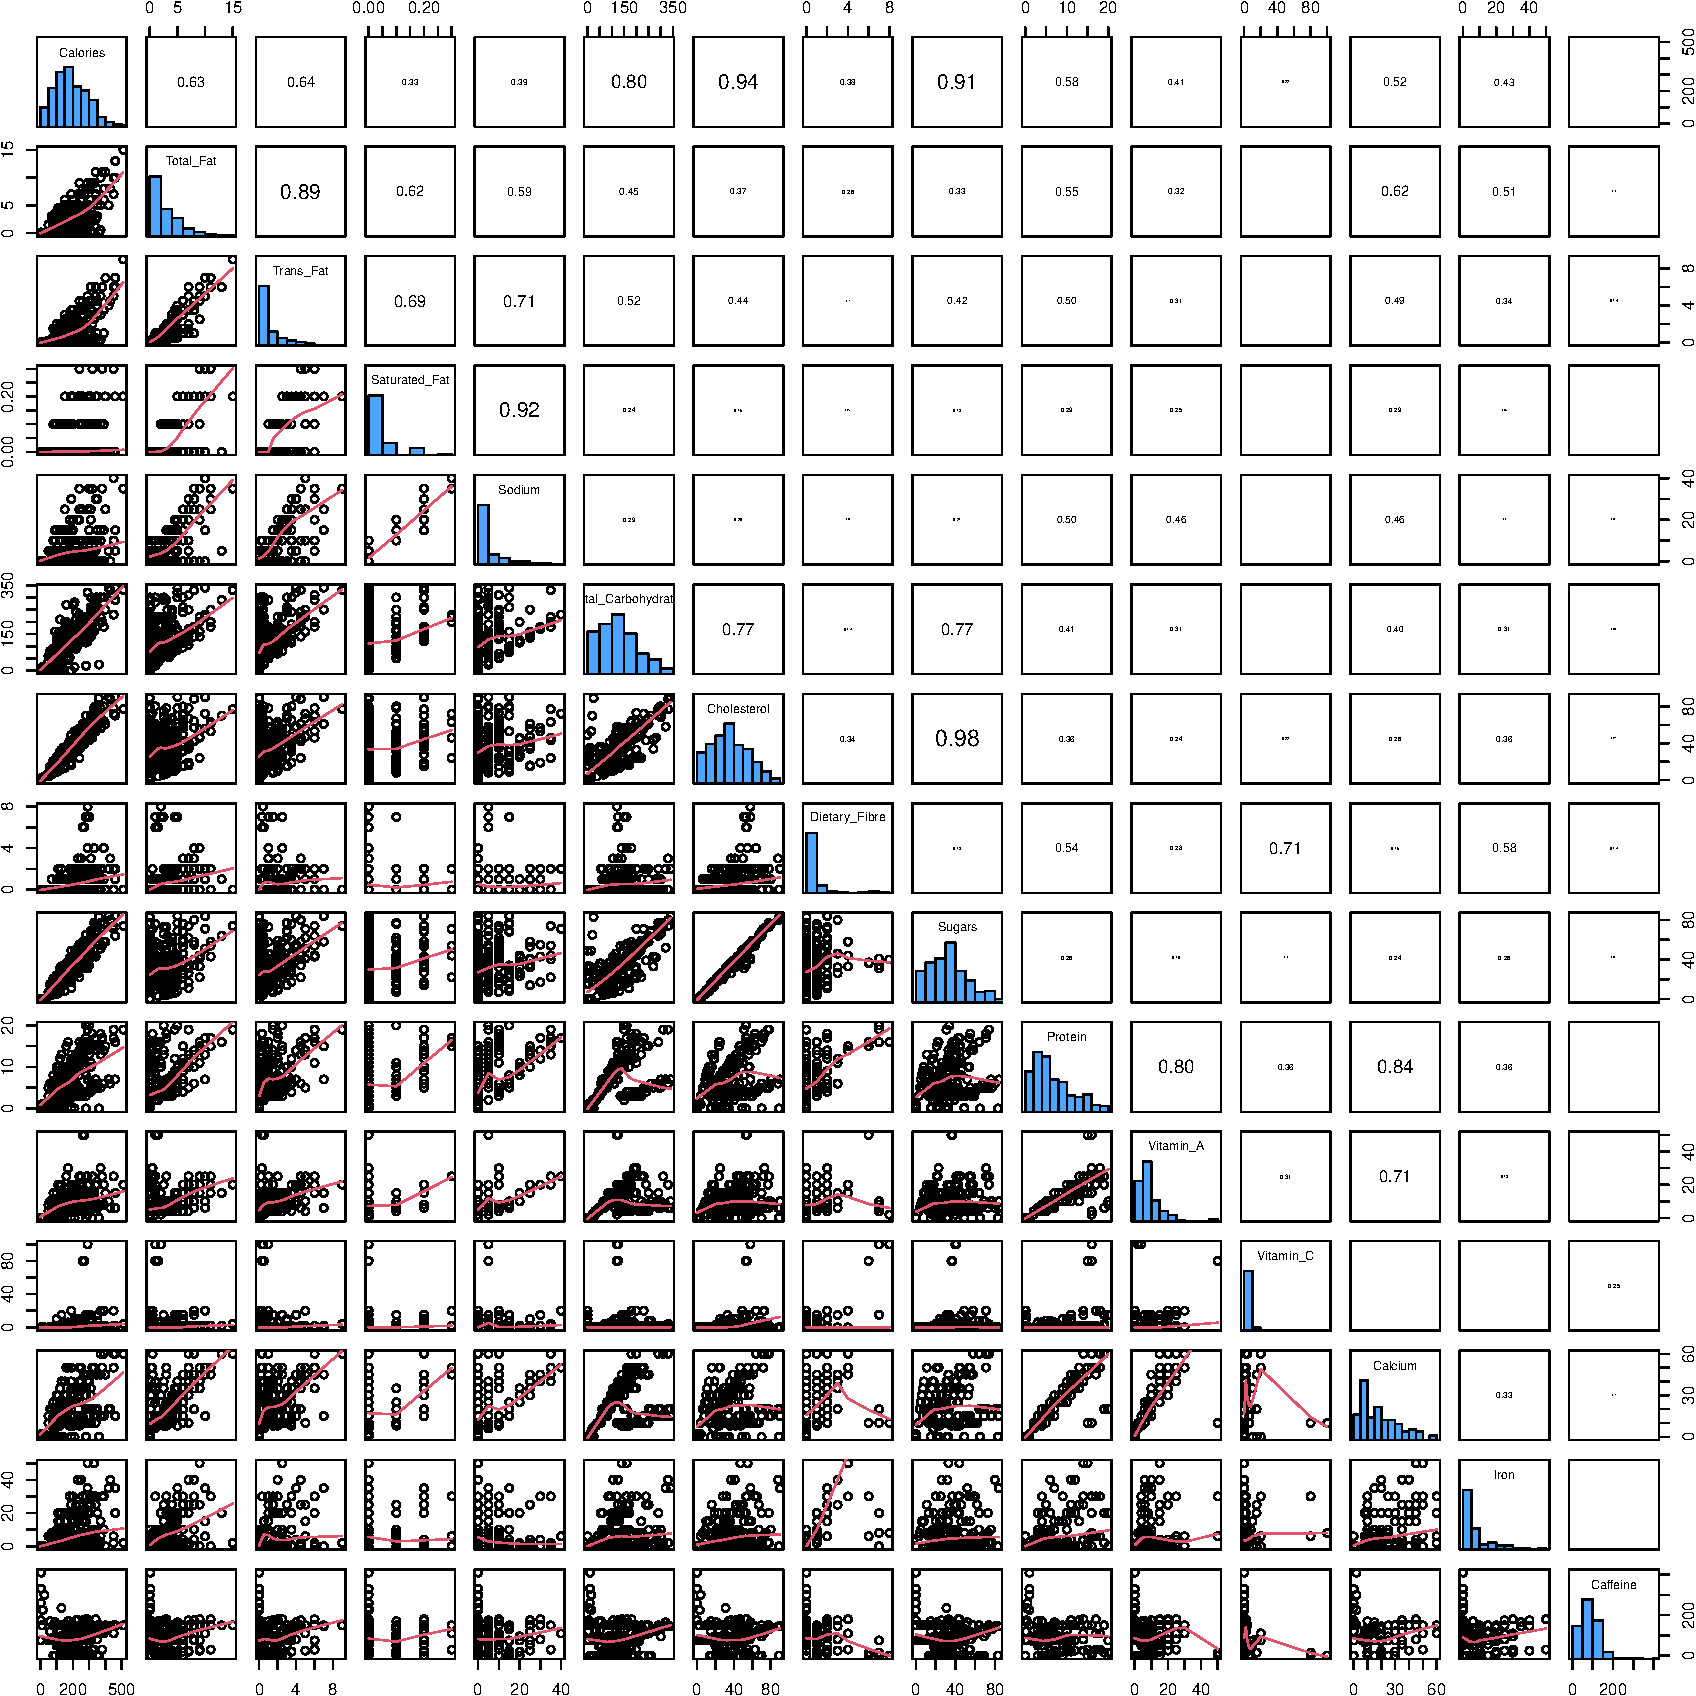
\includegraphics{Statistical_Learning_Final_Report_files/figure-latex/pairplot-1} \end{center}

ADD COMMENTS ON THE GRAPH

\subsection{Barplot}\label{barplot}

We will now plot the bar plots for our dataset. The primary use of bar
plots is to make comparisons between the amounts of different
categories. Indeed, each bar corresponds to a category and the height of
the bar represents the frequency or proportion of that category. These
graphs are commonly used for categorical data, or numerical data that
has been binned into categories.

\begin{Shaded}
\begin{Highlighting}[]
\FunctionTok{par}\NormalTok{(}\AttributeTok{mfrow =} \FunctionTok{c}\NormalTok{(}\DecValTok{5}\NormalTok{, }\DecValTok{3}\NormalTok{), }\AttributeTok{mar =} \FunctionTok{c}\NormalTok{(}\DecValTok{2}\NormalTok{, }\DecValTok{2}\NormalTok{, }\DecValTok{2}\NormalTok{, }\DecValTok{2}\NormalTok{))}
\ControlFlowTok{for}\NormalTok{ (i }\ControlFlowTok{in} \DecValTok{1}\SpecialCharTok{:}\FunctionTok{ncol}\NormalTok{(data\_num)) \{}
  \FunctionTok{barplot}\NormalTok{(}\FunctionTok{table}\NormalTok{(data\_num[, i]), }\AttributeTok{main =} \FunctionTok{colnames}\NormalTok{(data\_num)[i],}
          \AttributeTok{xlab =} \FunctionTok{colnames}\NormalTok{(data\_num)[i], }\AttributeTok{col =}\NormalTok{ col[i], }\AttributeTok{border =}\NormalTok{ col[i])}
\NormalTok{\}}
\end{Highlighting}
\end{Shaded}

\begin{center}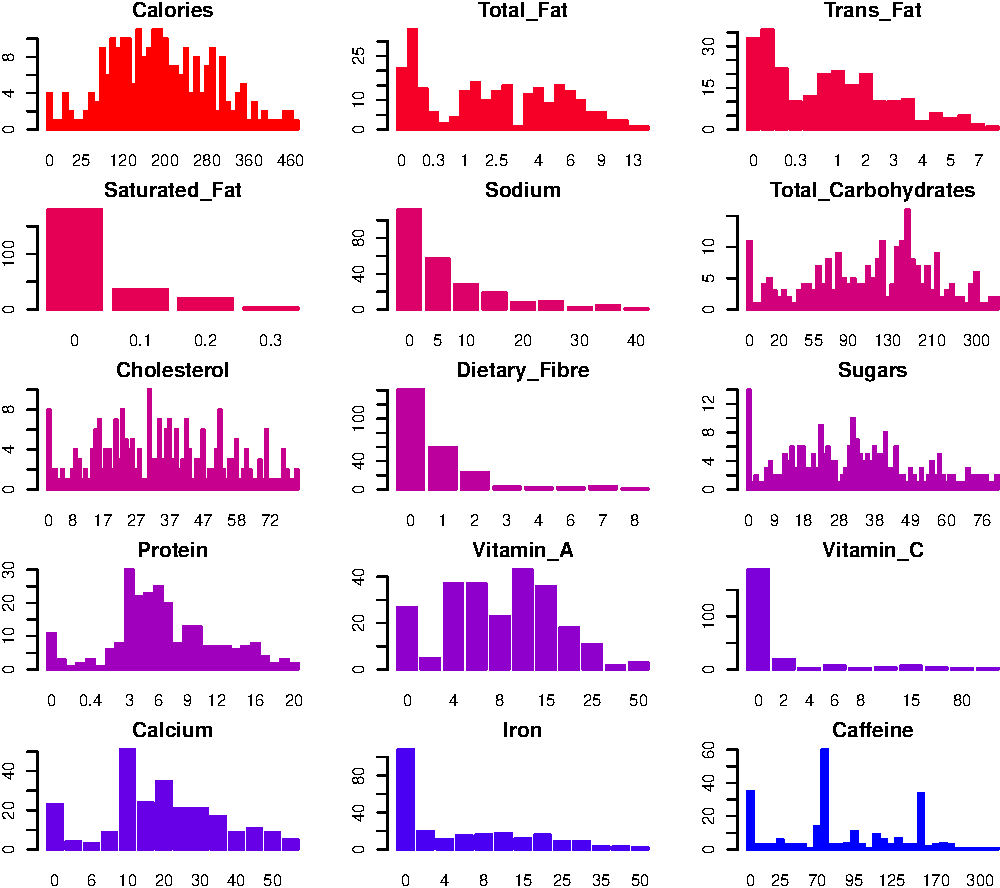
\includegraphics{Statistical_Learning_Final_Report_files/figure-latex/barplot-1} \end{center}

We can deduce some useful information by looking at these plots.

For example, we can notice that variables such as ``Saturated\_Fat'',
``Dietary\_Fibre'', ``Vitamin\_C'', and ``Iron'' are typically either
absent or present in small quantities in the beverages. In particular,
the frequency of these variables rapidly diminishes as their levels
increase. On the other hand, the variables ``Calories'', ``Total\_Fat'',
``Trans\_Fat'', and ``Total\_Carbohydrates'' show a wide range of values
across different beverage types, going from high levels in some
beverages to minimal amounts in others.

We can further observe that the distribution of ``Vitamin\_A'' appears
to be more evenly spread among the different levels in various
beverages, while instead ``Caffeine'' plot is interesting as it exhibits
three distinct peaks in frequency.

\subsubsection{Beverages Barplot}\label{beverages-barplot}

As previously anticipated, bar plots also allows us to see the
distribution of categorical variables like ``Beverage\_category'' and
``Beverage\_prep''. In this way we can identify the most frequently
occurring beverages and their preparation methods.

\begin{Shaded}
\begin{Highlighting}[]
\FunctionTok{par}\NormalTok{(}\AttributeTok{mfrow =} \FunctionTok{c}\NormalTok{(}\DecValTok{1}\NormalTok{, }\DecValTok{1}\NormalTok{), }\AttributeTok{mar =} \FunctionTok{c}\NormalTok{(}\DecValTok{8}\NormalTok{, }\DecValTok{2}\NormalTok{, }\DecValTok{2}\NormalTok{, }\DecValTok{2}\NormalTok{))}
\FunctionTok{barplot}\NormalTok{(}\FunctionTok{table}\NormalTok{(data}\SpecialCharTok{$}\NormalTok{Beverage\_category),}
        \AttributeTok{main =} \StringTok{"Distribution of Beverage Categories"}\NormalTok{,}
        \AttributeTok{ylab =} \StringTok{"Count"}\NormalTok{, }\AttributeTok{col =} \StringTok{"\#4ea5ff"}\NormalTok{, }\AttributeTok{las =} \DecValTok{2}\NormalTok{, }\AttributeTok{cex.names =} \FloatTok{0.6}\NormalTok{)}
\end{Highlighting}
\end{Shaded}

\begin{center}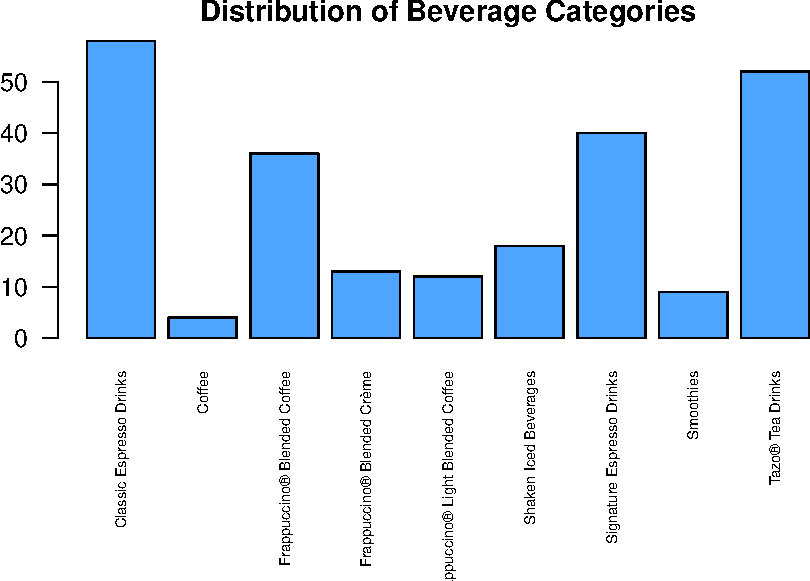
\includegraphics{Statistical_Learning_Final_Report_files/figure-latex/beverage_barplot-1} \end{center}

\begin{Shaded}
\begin{Highlighting}[]
\FunctionTok{barplot}\NormalTok{(}\FunctionTok{table}\NormalTok{(data}\SpecialCharTok{$}\NormalTok{Beverage\_prep),}
        \AttributeTok{main =} \StringTok{"Distribution of Beverage Preparation"}\NormalTok{,}
        \AttributeTok{ylab =} \StringTok{"Count"}\NormalTok{, }\AttributeTok{col =} \StringTok{"\#ff810f"}\NormalTok{, }\AttributeTok{las =} \DecValTok{2}\NormalTok{, }\AttributeTok{cex.names =} \FloatTok{0.6}\NormalTok{)}
\end{Highlighting}
\end{Shaded}

\begin{center}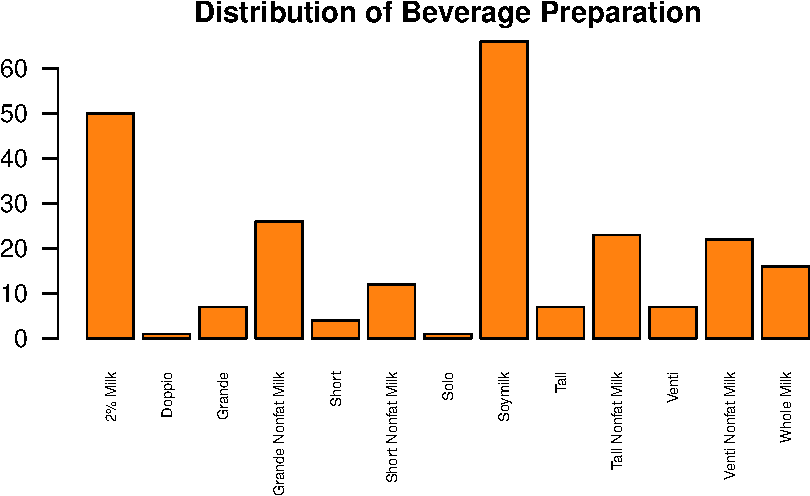
\includegraphics{Statistical_Learning_Final_Report_files/figure-latex/beverage_barplot-2} \end{center}

At this point, we aim to compare the total calorie content among
different beverage categories. To do so, we first aggregate the data to
obtain the total calories for each beverage category. Secondly, we
construct a bar plot to visually represent the results.

\begin{Shaded}
\begin{Highlighting}[]
\FunctionTok{par}\NormalTok{(}\AttributeTok{mfrow =} \FunctionTok{c}\NormalTok{(}\DecValTok{1}\NormalTok{, }\DecValTok{1}\NormalTok{), }\AttributeTok{mar =} \FunctionTok{c}\NormalTok{(}\DecValTok{8}\NormalTok{, }\DecValTok{4}\NormalTok{, }\DecValTok{2}\NormalTok{, }\DecValTok{2}\NormalTok{))}
\NormalTok{total\_calories\_by\_category }\OtherTok{\textless{}{-}} \FunctionTok{aggregate}\NormalTok{(Calories }\SpecialCharTok{\textasciitilde{}}\NormalTok{ Beverage\_category,}
                                        \AttributeTok{data =}\NormalTok{ data\_cleaned, sum)}
\FunctionTok{barplot}\NormalTok{(}\AttributeTok{height =}\NormalTok{ total\_calories\_by\_category}\SpecialCharTok{$}\NormalTok{Calories,}
        \AttributeTok{names.arg =}\NormalTok{ total\_calories\_by\_category}\SpecialCharTok{$}\NormalTok{Beverage\_category,}
        \AttributeTok{main =} \StringTok{"Total Calories by Beverage Category"}\NormalTok{,}
        \AttributeTok{ylab =} \StringTok{"Total Calories"}\NormalTok{, }\AttributeTok{col =} \StringTok{"\#4ea5ff"}\NormalTok{, }\AttributeTok{las =} \DecValTok{2}\NormalTok{, }\AttributeTok{cex.names =} \FloatTok{0.6}\NormalTok{)}
\end{Highlighting}
\end{Shaded}

\begin{center}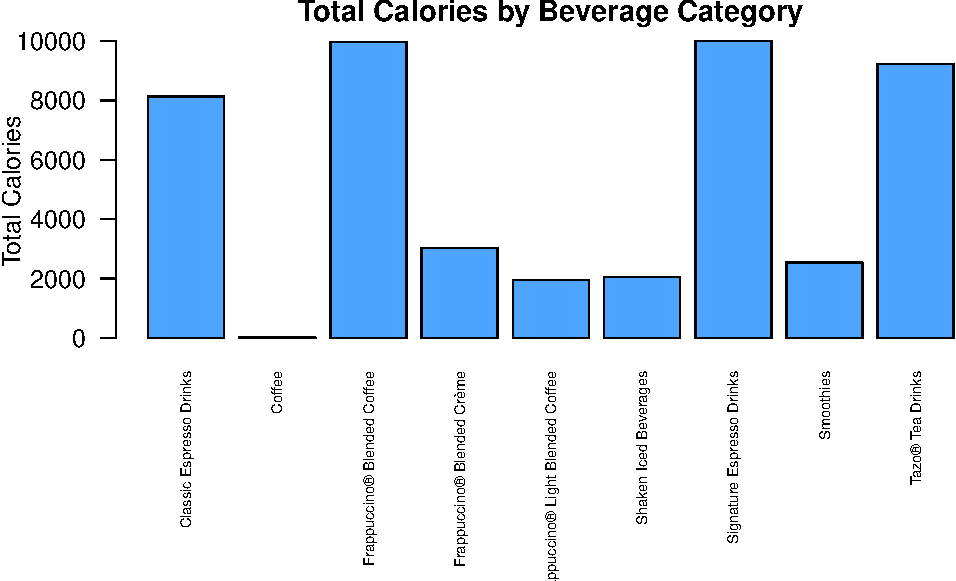
\includegraphics{Statistical_Learning_Final_Report_files/figure-latex/total_calories-1} \end{center}

Similarly, we compare the total sugars for each beverage preparation,
gathering data to obtain the total sugars for each preparation of
beverage and successively creating a bar plot.

\begin{Shaded}
\begin{Highlighting}[]
\FunctionTok{par}\NormalTok{(}\AttributeTok{mfrow =} \FunctionTok{c}\NormalTok{(}\DecValTok{1}\NormalTok{, }\DecValTok{1}\NormalTok{), }\AttributeTok{mar =} \FunctionTok{c}\NormalTok{(}\DecValTok{8}\NormalTok{, }\DecValTok{4}\NormalTok{, }\DecValTok{2}\NormalTok{, }\DecValTok{2}\NormalTok{))}
\NormalTok{total\_sugar\_by\_prep }\OtherTok{\textless{}{-}} \FunctionTok{aggregate}\NormalTok{(Total\_Carbohydrates }\SpecialCharTok{\textasciitilde{}}\NormalTok{ Beverage\_prep,}
                                 \AttributeTok{data =}\NormalTok{ data\_cleaned, sum)}
\FunctionTok{barplot}\NormalTok{(}\AttributeTok{height =}\NormalTok{ total\_sugar\_by\_prep}\SpecialCharTok{$}\NormalTok{Total\_Carbohydrates,}
        \AttributeTok{names.arg =}\NormalTok{ total\_sugar\_by\_prep}\SpecialCharTok{$}\NormalTok{Beverage\_prep,}
        \AttributeTok{main =} \StringTok{"Total Sugars by Beverage Preparation"}\NormalTok{,}
        \AttributeTok{ylab =} \StringTok{"Total Sugars (g)"}\NormalTok{, }\AttributeTok{col =} \StringTok{"\#ff810f"}\NormalTok{, }\AttributeTok{las =} \DecValTok{2}\NormalTok{, }\AttributeTok{cex.names =} \FloatTok{0.6}\NormalTok{)}
\end{Highlighting}
\end{Shaded}

\begin{center}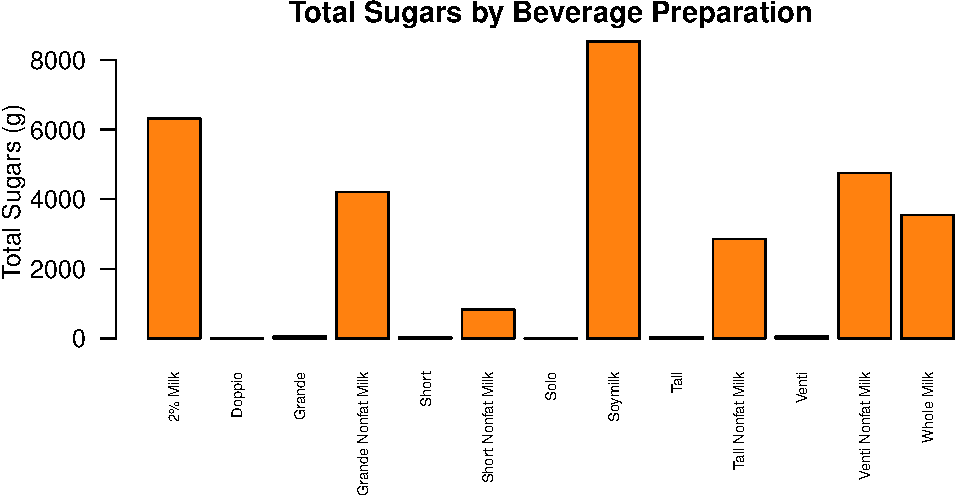
\includegraphics{Statistical_Learning_Final_Report_files/figure-latex/total_sugars-1} \end{center}

\subsection{Boxplot}\label{boxplot}

We will plot a boxplot of the data. The boxplot is a graphical
representation of the data that displays the distribution of the data,
including the median, quartiles, and outliers. This visualization helps
us to identify the spread and variability of the data.

\begin{Shaded}
\begin{Highlighting}[]
\FunctionTok{par}\NormalTok{(}\AttributeTok{mfrow =} \FunctionTok{c}\NormalTok{(}\DecValTok{3}\NormalTok{, }\DecValTok{5}\NormalTok{), }\AttributeTok{mar =} \FunctionTok{c}\NormalTok{(}\DecValTok{2}\NormalTok{, }\DecValTok{2}\NormalTok{, }\DecValTok{2}\NormalTok{, }\DecValTok{2}\NormalTok{))}
\ControlFlowTok{for}\NormalTok{ (i }\ControlFlowTok{in} \DecValTok{1}\SpecialCharTok{:}\FunctionTok{ncol}\NormalTok{(data\_num)) \{}
  \FunctionTok{boxplot}\NormalTok{(data\_num[, i], }\AttributeTok{main =} \FunctionTok{colnames}\NormalTok{(data\_num)[i],}
          \AttributeTok{xlab =} \FunctionTok{colnames}\NormalTok{(data\_num)[i], }\AttributeTok{col =}\NormalTok{ col[i])}
\NormalTok{\}}
\end{Highlighting}
\end{Shaded}

\begin{center}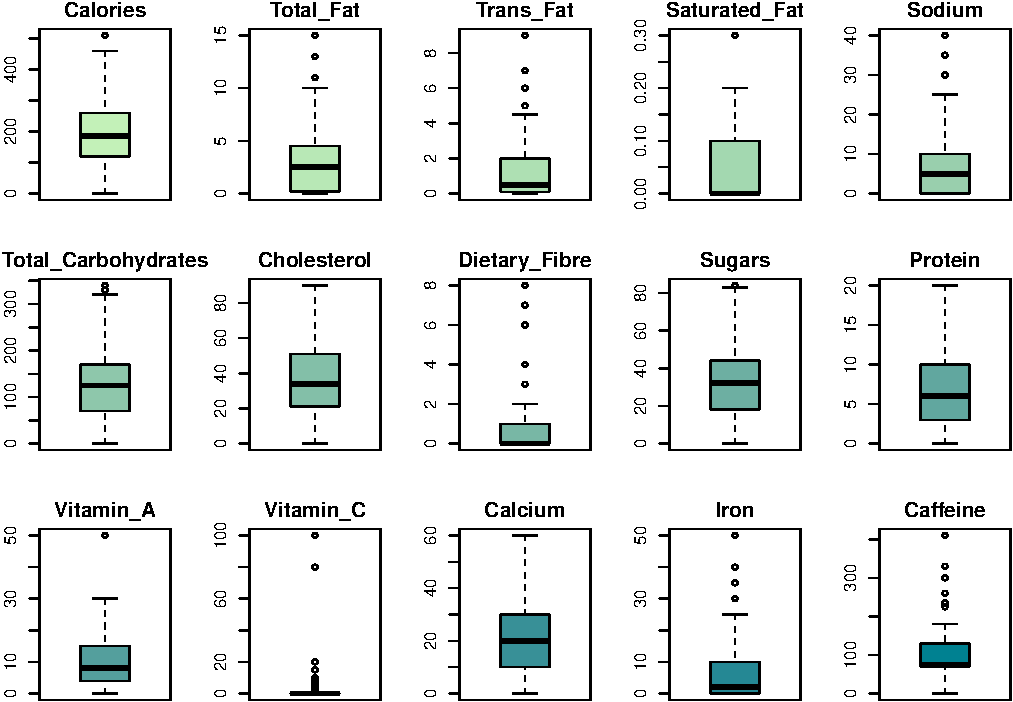
\includegraphics{Statistical_Learning_Final_Report_files/figure-latex/boxplot-1} \end{center}

\subsection{Scatterplot}\label{scatterplot}

We will plot a scatterplot of the data. The scatterplot is a graphical
representation of the data that displays the relationship between two
variables. This visualization helps us to identify patterns and
correlations between the variables.

We create a scatterplot to compare the amounts of calories and fat for
each categories of bevarage. We assign distinct colors to each beverage
category and create a legend to identify each category.

\begin{Shaded}
\begin{Highlighting}[]
\CommentTok{\# Set the variable as factor}
\NormalTok{data\_cleaned}\SpecialCharTok{$}\NormalTok{Beverage\_category }\OtherTok{\textless{}{-}} \FunctionTok{as.factor}\NormalTok{(data\_cleaned}\SpecialCharTok{$}\NormalTok{Beverage\_category)}
\NormalTok{colors }\OtherTok{\textless{}{-}} \FunctionTok{rainbow}\NormalTok{(}\FunctionTok{length}\NormalTok{(}\FunctionTok{unique}\NormalTok{(data\_cleaned}\SpecialCharTok{$}\NormalTok{Beverage\_category)))}
\NormalTok{color\_map }\OtherTok{\textless{}{-}} \FunctionTok{setNames}\NormalTok{(colors, }\FunctionTok{levels}\NormalTok{(data\_cleaned}\SpecialCharTok{$}\NormalTok{Beverage\_category))}
\FunctionTok{par}\NormalTok{(}\AttributeTok{mfrow =} \FunctionTok{c}\NormalTok{(}\DecValTok{1}\NormalTok{, }\DecValTok{1}\NormalTok{))}
\FunctionTok{plot}\NormalTok{(data\_cleaned}\SpecialCharTok{$}\NormalTok{Calories, }
\NormalTok{     data\_cleaned}\SpecialCharTok{$}\NormalTok{Total\_Fat\_g,}
     \AttributeTok{col =}\NormalTok{ color\_map[data\_cleaned}\SpecialCharTok{$}\NormalTok{Beverage\_category],}
     \AttributeTok{pch =} \DecValTok{19}\NormalTok{, }\AttributeTok{xlab =} \StringTok{"Calories"}\NormalTok{, }\AttributeTok{ylab =} \StringTok{"Total Fat (g)"}\NormalTok{,}
     \AttributeTok{main =} \StringTok{"Calories vs Total Fat"}\NormalTok{)}
\FunctionTok{legend}\NormalTok{(}\StringTok{"topleft"}\NormalTok{, }\AttributeTok{legend =} \FunctionTok{levels}\NormalTok{(data\_cleaned}\SpecialCharTok{$}\NormalTok{Beverage\_category), }
       \AttributeTok{col =}\NormalTok{ colors, }\AttributeTok{cex =} \FloatTok{0.4}\NormalTok{, }\AttributeTok{pch =} \DecValTok{19}\NormalTok{)}
\end{Highlighting}
\end{Shaded}

\begin{center}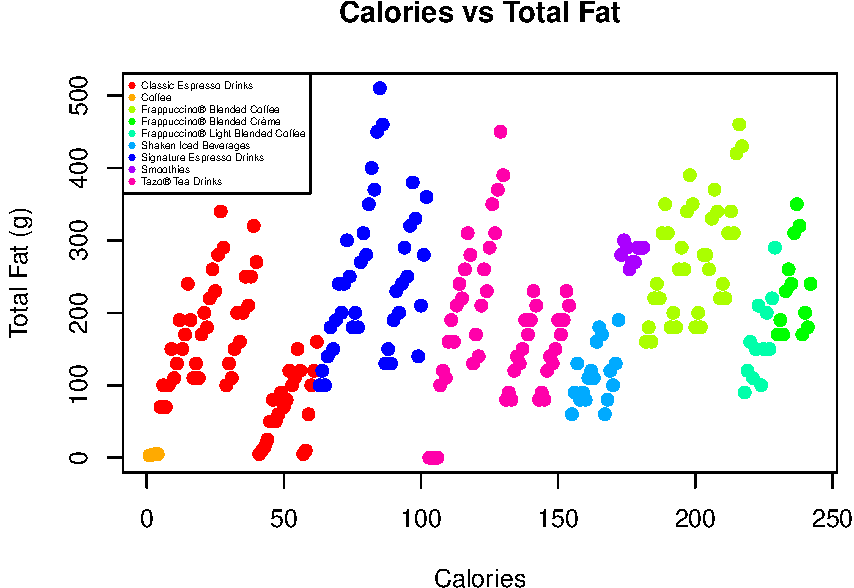
\includegraphics{Statistical_Learning_Final_Report_files/figure-latex/fat_comparison-1} \end{center}

\begin{Shaded}
\begin{Highlighting}[]
\CommentTok{\# Numeric variable {-}\textgreater{} calculate density}
\NormalTok{total\_fat\_density }\OtherTok{\textless{}{-}} \FunctionTok{density}\NormalTok{(data\_cleaned}\SpecialCharTok{$}\NormalTok{Total\_Fat)}
\NormalTok{trans\_fat\_density }\OtherTok{\textless{}{-}} \FunctionTok{density}\NormalTok{(data\_cleaned}\SpecialCharTok{$}\NormalTok{Trans\_Fat)}
\FunctionTok{plot}\NormalTok{(total\_fat\_density, }\AttributeTok{col =} \StringTok{"\#4ea5ff"}\NormalTok{,}
     \AttributeTok{main =} \StringTok{"Comparison of Total Fat and Trans Fat Distributions"}\NormalTok{, }
     \AttributeTok{xlab =} \StringTok{"Fat Content (g)"}\NormalTok{, }\AttributeTok{ylab =} \StringTok{"Density"}\NormalTok{, }
     \AttributeTok{ylim =} \FunctionTok{c}\NormalTok{(}\DecValTok{0}\NormalTok{, }\FunctionTok{max}\NormalTok{(total\_fat\_density}\SpecialCharTok{$}\NormalTok{y, trans\_fat\_density}\SpecialCharTok{$}\NormalTok{y)),}
     \AttributeTok{xlim =} \FunctionTok{range}\NormalTok{(data\_cleaned}\SpecialCharTok{$}\NormalTok{Total\_Fat, data\_cleaned}\SpecialCharTok{$}\NormalTok{Trans\_Fat), }
     \AttributeTok{lwd =} \DecValTok{2}\NormalTok{, }\AttributeTok{lty =} \DecValTok{1}\NormalTok{)}
\FunctionTok{lines}\NormalTok{(trans\_fat\_density, }\AttributeTok{col =} \StringTok{"\#ff810f"}\NormalTok{, }\AttributeTok{lwd =} \DecValTok{2}\NormalTok{, }\AttributeTok{lty =} \DecValTok{1}\NormalTok{)}
\FunctionTok{legend}\NormalTok{(}\StringTok{"topright"}\NormalTok{, }\AttributeTok{legend =} \FunctionTok{c}\NormalTok{(}\StringTok{"Total Fat"}\NormalTok{, }\StringTok{"Trans Fat"}\NormalTok{),}
       \AttributeTok{col =} \FunctionTok{c}\NormalTok{(}\StringTok{"\#4ea5ff"}\NormalTok{, }\StringTok{"\#ff810f"}\NormalTok{), }\AttributeTok{lwd =} \DecValTok{2}\NormalTok{, }\AttributeTok{lty =} \DecValTok{1}\NormalTok{)}
\end{Highlighting}
\end{Shaded}

\begin{center}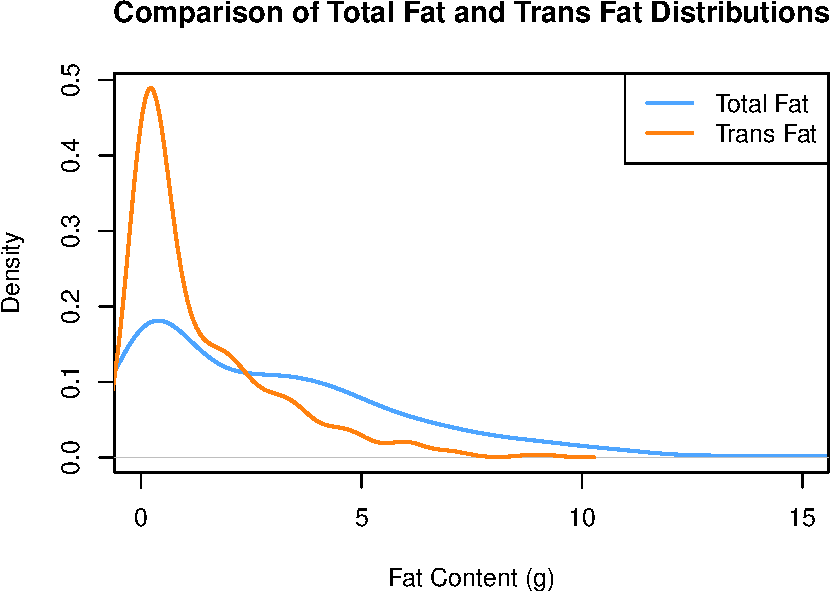
\includegraphics{Statistical_Learning_Final_Report_files/figure-latex/fat_comparison-2} \end{center}

Create scatterplot to look into relantionship between calories and other
variables. We will plot the relationship between calories and sodium,
protein, vitamin C and fiber.

\begin{Shaded}
\begin{Highlighting}[]
\FunctionTok{par}\NormalTok{(}\AttributeTok{mfrow =} \FunctionTok{c}\NormalTok{(}\DecValTok{2}\NormalTok{, }\DecValTok{2}\NormalTok{), }\AttributeTok{mar =} \FunctionTok{c}\NormalTok{(}\DecValTok{4}\NormalTok{, }\DecValTok{4}\NormalTok{, }\DecValTok{2}\NormalTok{, }\DecValTok{2}\NormalTok{))}
\FunctionTok{with}\NormalTok{(data\_cleaned, \{}
  \FunctionTok{plot}\NormalTok{(Calories, Sodium , }\AttributeTok{main =} \StringTok{"Relation between Calories and Sodium"}\NormalTok{,}
       \AttributeTok{xlab =} \StringTok{"Calories"}\NormalTok{, }\AttributeTok{ylab =} \StringTok{"Sodium (mg)"}\NormalTok{, }\AttributeTok{col =}\NormalTok{ col[}\DecValTok{1}\NormalTok{])}
  \FunctionTok{plot}\NormalTok{(Calories, Protein , }\AttributeTok{main =} \StringTok{"Relation between Calories and Protein"}\NormalTok{,}
       \AttributeTok{xlab =} \StringTok{"Calories"}\NormalTok{, }\AttributeTok{ylab =} \StringTok{"Protein (g)"}\NormalTok{, }\AttributeTok{col =}\NormalTok{ col[}\DecValTok{5}\NormalTok{])}
  \FunctionTok{plot}\NormalTok{(Calories, Vitamin\_C , }\AttributeTok{main =} \StringTok{"Relation between Calories and Vitamin C"}\NormalTok{,}
       \AttributeTok{xlab =} \StringTok{"Calories"}\NormalTok{, }\AttributeTok{ylab =} \StringTok{"Vitamin C (mg)"}\NormalTok{, }\AttributeTok{col =}\NormalTok{ col[}\DecValTok{10}\NormalTok{])}
  \FunctionTok{plot}\NormalTok{(Calories, Cholesterol , }\AttributeTok{main =} \StringTok{"Relation between Calories and Fiber"}\NormalTok{,}
       \AttributeTok{xlab =} \StringTok{"Calories"}\NormalTok{, }\AttributeTok{ylab =} \StringTok{"Fiber (g)"}\NormalTok{, }\AttributeTok{col =}\NormalTok{ col[}\DecValTok{15}\NormalTok{])}
\NormalTok{\})}
\end{Highlighting}
\end{Shaded}

\begin{center}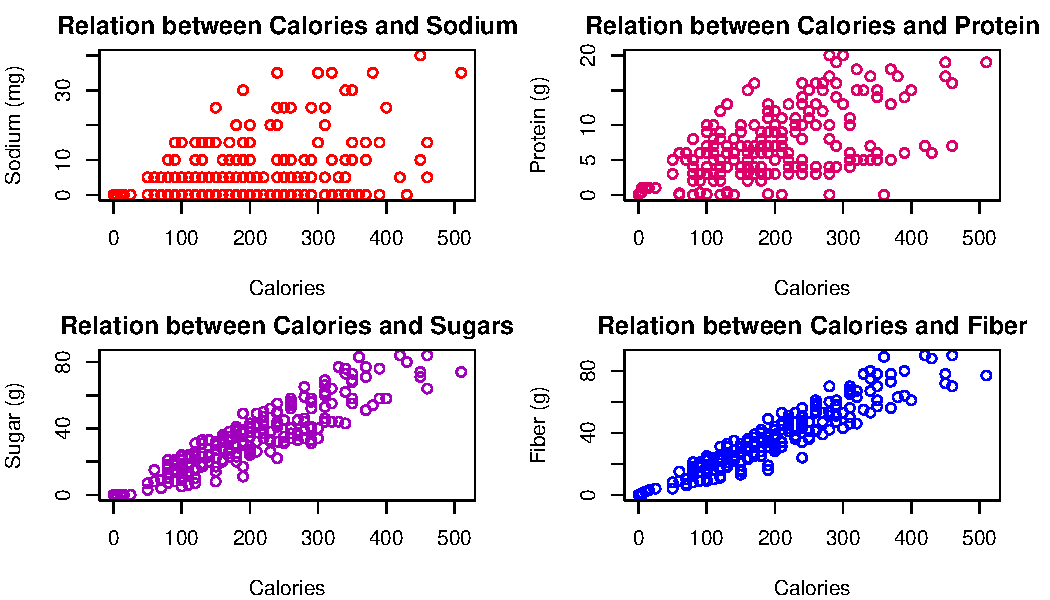
\includegraphics{Statistical_Learning_Final_Report_files/figure-latex/scatterplot-1} \end{center}

There's increase in every feature with increase in calories. Features
like proteins and fiber rapidly increase, instead vitamin and
cholesterol more flat growing. Confirmed by correlation coefficients

ADD COMMENTS ON THE GRAPH

\section{Regression Analysis}\label{regression-analysis}

\subsection{Linear Regression}\label{linear-regression}

Linear regression model to predict the amount of calories based on the
amount of the other variables We use the lm() function to fit a linear
regression model

\begin{Shaded}
\begin{Highlighting}[]
\NormalTok{lm\_model }\OtherTok{\textless{}{-}} \FunctionTok{lm}\NormalTok{(y }\SpecialCharTok{\textasciitilde{}}\NormalTok{ ., }\AttributeTok{data =}\NormalTok{ data\_num\_)}
\FunctionTok{summary}\NormalTok{(lm\_model)}
\end{Highlighting}
\end{Shaded}

\begin{verbatim}
## 
## Call:
## lm(formula = y ~ ., data = data_num_)
## 
## Residuals:
##      Min       1Q   Median       3Q      Max 
## -14.0233  -3.3009  -0.3806   3.0039  21.9404 
## 
## Coefficients:
##                      Estimate Std. Error t value Pr(>|t|)    
## (Intercept)          0.252316   0.952833   0.265  0.79140    
## Total_Fat           11.143733   0.532812  20.915  < 2e-16 ***
## Trans_Fat           -2.477820   0.809270  -3.062  0.00247 ** 
## Saturated_Fat       -9.816317  18.143619  -0.541  0.58901    
## Sodium              -0.279257   0.167487  -1.667  0.09683 .  
## Total_Carbohydrates  0.020972   0.007420   2.826  0.00513 ** 
## Cholesterol          2.829543   0.340268   8.316 8.43e-15 ***
## Dietary_Fibre        1.534913   0.942106   1.629  0.10465    
## Sugars               1.131045   0.348234   3.248  0.00134 ** 
## Protein              2.218895   0.510445   4.347 2.08e-05 ***
## Vitamin_A            0.162307   0.083662   1.940  0.05361 .  
## Vitamin_C            0.147669   0.047675   3.097  0.00220 ** 
## Calcium              0.462193   0.142257   3.249  0.00133 ** 
## Iron                -0.649101   0.070666  -9.185  < 2e-16 ***
## Caffeine             0.013513   0.005826   2.319  0.02126 *  
## ---
## Signif. codes:  0 '***' 0.001 '**' 0.01 '*' 0.05 '.' 0.1 ' ' 1
## 
## Residual standard error: 5.126 on 227 degrees of freedom
## Multiple R-squared:  0.9977, Adjusted R-squared:  0.9975 
## F-statistic:  6915 on 14 and 227 DF,  p-value: < 2.2e-16
\end{verbatim}

\begin{Shaded}
\begin{Highlighting}[]
\FunctionTok{par}\NormalTok{(}\AttributeTok{mfrow =} \FunctionTok{c}\NormalTok{(}\DecValTok{2}\NormalTok{, }\DecValTok{2}\NormalTok{), }\AttributeTok{mar =} \FunctionTok{c}\NormalTok{(}\DecValTok{2}\NormalTok{, }\DecValTok{2}\NormalTok{, }\DecValTok{2}\NormalTok{, }\DecValTok{2}\NormalTok{))}
\FunctionTok{plot}\NormalTok{(lm\_model)}
\end{Highlighting}
\end{Shaded}

\begin{center}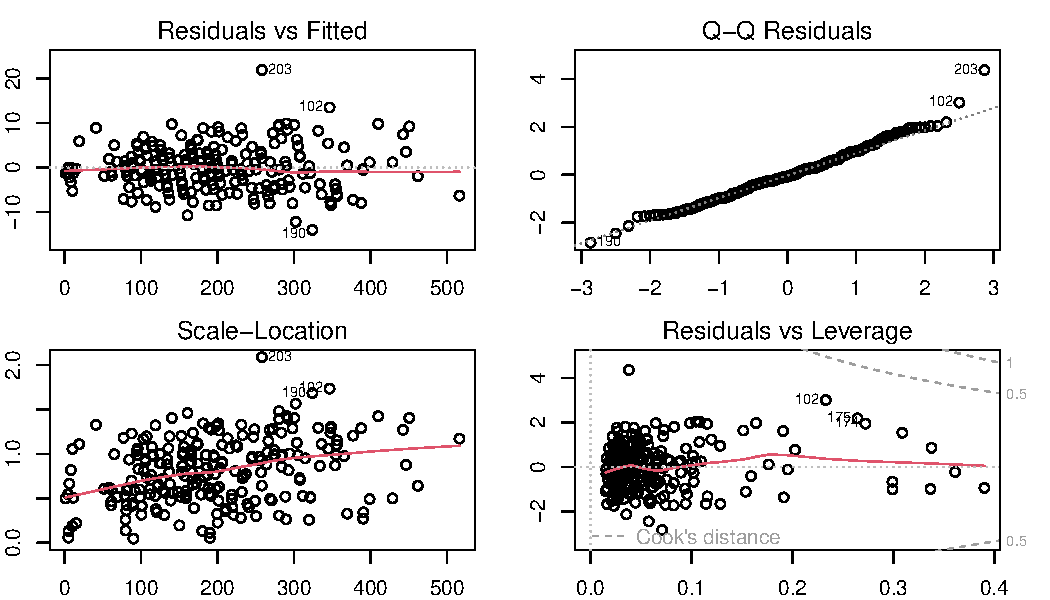
\includegraphics{Statistical_Learning_Final_Report_files/figure-latex/linear_regression-1} \end{center}

\begin{Shaded}
\begin{Highlighting}[]
\FunctionTok{kable}\NormalTok{(}\FunctionTok{data.frame}\NormalTok{(}\AttributeTok{AIC =} \FunctionTok{AIC}\NormalTok{(lm\_model), }\AttributeTok{BIC =} \FunctionTok{BIC}\NormalTok{(lm\_model),}
                 \AttributeTok{R\_squared =} \FunctionTok{summary}\NormalTok{(lm\_model)}\SpecialCharTok{$}\NormalTok{r.squared), }
      \AttributeTok{caption =} \StringTok{"Model evaluation metrics"}\NormalTok{)}
\end{Highlighting}
\end{Shaded}

\begin{longtable}[]{@{}rrr@{}}
\caption{Model evaluation metrics}\tabularnewline
\toprule\noalign{}
AIC & BIC & R\_squared \\
\midrule\noalign{}
\endfirsthead
\toprule\noalign{}
AIC & BIC & R\_squared \\
\midrule\noalign{}
\endhead
\bottomrule\noalign{}
\endlastfoot
1494.304 & 1550.127 & 0.9976608 \\
\end{longtable}

\begin{Shaded}
\begin{Highlighting}[]
\FunctionTok{kable}\NormalTok{(}\FunctionTok{data.frame}\NormalTok{(}\AttributeTok{VIF =} \FunctionTok{vif}\NormalTok{(lm\_model)),}
      \AttributeTok{caption =} \StringTok{"VIF values for the linear regression model"}\NormalTok{)}
\end{Highlighting}
\end{Shaded}

\begin{longtable}[]{@{}lr@{}}
\caption{VIF values for the linear regression model}\tabularnewline
\toprule\noalign{}
& VIF \\
\midrule\noalign{}
\endfirsthead
\toprule\noalign{}
& VIF \\
\midrule\noalign{}
\endhead
\bottomrule\noalign{}
\endlastfoot
Total\_Fat & 22.572405 \\
Trans\_Fat & 16.160511 \\
Saturated\_Fat & 15.381749 \\
Sodium & 19.162550 \\
Total\_Carbohydrates & 3.420278 \\
Cholesterol & 459.209279 \\
Dietary\_Fibre & 17.019469 \\
Sugars & 432.962393 \\
Protein & 56.714696 \\
Vitamin\_A & 4.209673 \\
Vitamin\_C & 4.335768 \\
Calcium & 39.251753 \\
Iron & 5.036421 \\
Caffeine & 1.185411 \\
\end{longtable}

The model has a low AIC and BIC values, the R-squared value is 0.997 so
the model is a good fit for the data. However as we can see from the
\emph{Table 2} e have a problem with multicollinearity, the VIF values
are high for some variables, so we have to act on the data to solve this
problem

We try to standardize the data using a logaritmic transformation

\begin{Shaded}
\begin{Highlighting}[]
\NormalTok{std\_data\_log }\OtherTok{\textless{}{-}} \FunctionTok{scale}\NormalTok{(}\FunctionTok{log}\NormalTok{(data\_num }\SpecialCharTok{+} \DecValTok{1}\NormalTok{)) }\CommentTok{\# Standardize the data}
\NormalTok{std\_data\_log\_df }\OtherTok{\textless{}{-}} \FunctionTok{as.data.frame}\NormalTok{(std\_data\_log) }\CommentTok{\# Set as dataframe}
\NormalTok{mod\_log\_tr }\OtherTok{\textless{}{-}} \FunctionTok{lm}\NormalTok{(Calories }\SpecialCharTok{\textasciitilde{}}\NormalTok{ ., }\AttributeTok{data =}\NormalTok{ std\_data\_log\_df)}
\FunctionTok{kable}\NormalTok{(}\FunctionTok{data.frame}\NormalTok{(}\AttributeTok{AIC =} \FunctionTok{AIC}\NormalTok{(mod\_log\_tr), }\AttributeTok{BIC =} \FunctionTok{BIC}\NormalTok{(mod\_log\_tr),}
                 \AttributeTok{R\_squared =} \FunctionTok{summary}\NormalTok{(mod\_log\_tr)}\SpecialCharTok{$}\NormalTok{r.squared), }
      \AttributeTok{caption =} \StringTok{"Model evaluation metrics for the log transformed data"}\NormalTok{)}
\end{Highlighting}
\end{Shaded}

\begin{longtable}[]{@{}rrr@{}}
\caption{Model evaluation metrics for the log transformed
data}\tabularnewline
\toprule\noalign{}
AIC & BIC & R\_squared \\
\midrule\noalign{}
\endfirsthead
\toprule\noalign{}
AIC & BIC & R\_squared \\
\midrule\noalign{}
\endhead
\bottomrule\noalign{}
\endlastfoot
-53.42411 & 2.398897 & 0.9586932 \\
\end{longtable}

\begin{Shaded}
\begin{Highlighting}[]
\FunctionTok{kable}\NormalTok{(}\FunctionTok{data.frame}\NormalTok{(}\AttributeTok{VIF =} \FunctionTok{vif}\NormalTok{(mod\_log\_tr)),}
      \AttributeTok{caption =} \StringTok{"VIF values for the log transformed data"}\NormalTok{)}
\end{Highlighting}
\end{Shaded}

\begin{longtable}[]{@{}lr@{}}
\caption{VIF values for the log transformed data}\tabularnewline
\toprule\noalign{}
& VIF \\
\midrule\noalign{}
\endfirsthead
\toprule\noalign{}
& VIF \\
\midrule\noalign{}
\endhead
\bottomrule\noalign{}
\endlastfoot
Total\_Fat & 12.049669 \\
Trans\_Fat & 10.577306 \\
Saturated\_Fat & 4.528080 \\
Sodium & 5.817088 \\
Total\_Carbohydrates & 4.363628 \\
Cholesterol & 39.988684 \\
Dietary\_Fibre & 7.115085 \\
Sugars & 38.415586 \\
Protein & 31.007121 \\
Vitamin\_A & 13.647581 \\
Vitamin\_C & 2.196674 \\
Calcium & 25.873742 \\
Iron & 4.582594 \\
Caffeine & 1.310005 \\
\end{longtable}

\begin{Shaded}
\begin{Highlighting}[]
\FunctionTok{par}\NormalTok{(}\AttributeTok{mfrow =} \FunctionTok{c}\NormalTok{(}\DecValTok{2}\NormalTok{, }\DecValTok{2}\NormalTok{), }\AttributeTok{mar =} \FunctionTok{c}\NormalTok{(}\DecValTok{2}\NormalTok{, }\DecValTok{2}\NormalTok{, }\DecValTok{2}\NormalTok{, }\DecValTok{2}\NormalTok{))}
\FunctionTok{plot}\NormalTok{(mod\_log\_tr)}
\end{Highlighting}
\end{Shaded}

\begin{center}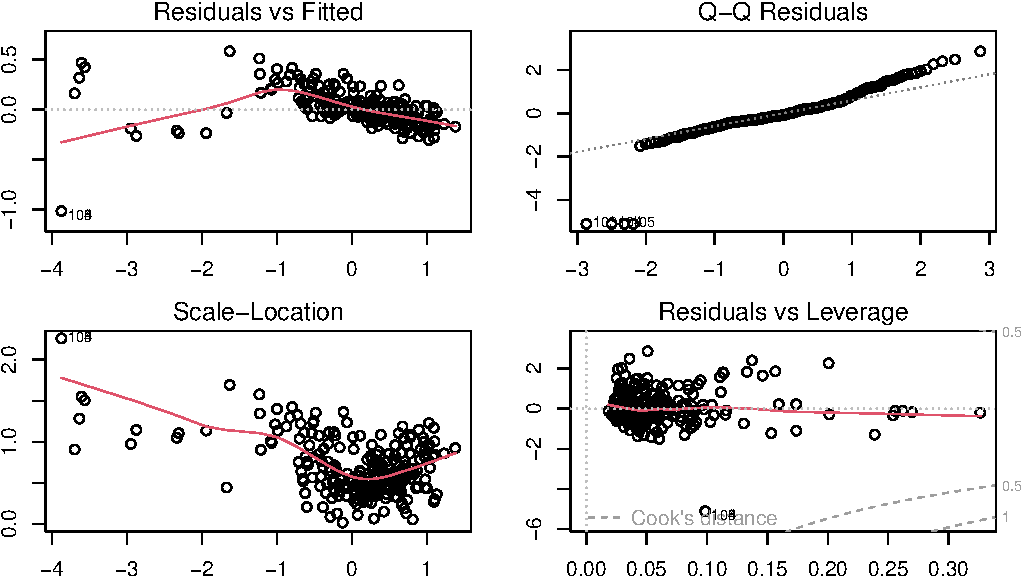
\includegraphics{Statistical_Learning_Final_Report_files/figure-latex/vif-1} \end{center}

The model has a low AIC and BIC values, the R-squared value is 0.95 so
the model is a good fit for the data. However we have still
collinearity, so we try to use another model.

\subsection{Lasso Regression}\label{lasso-regression}

We use the glmnet package to fit a lasso regression model. Lasso
regression is a type of linear regression that uses L1 regularization to
penalize the coefficients of the model. This helps to prevent
overfitting and select the most important features in the data.

First we standardize the data and then we fit the lasso regression model
using the cv.glmnet() function. We use cross-validation to select the
optimal lambda value for the model. The lambda value that minimizes the
mean squared error (MSE) is selected as the optimal lambda value. The
optimal lambda value is used to fit the final lasso regression model.

\begin{Shaded}
\begin{Highlighting}[]
\NormalTok{std\_data }\OtherTok{\textless{}{-}} \FunctionTok{as.data.frame}\NormalTok{(}\FunctionTok{scale}\NormalTok{(data\_num)) }\CommentTok{\# Standardize the data}
\NormalTok{mod\_lasso }\OtherTok{\textless{}{-}} \FunctionTok{cv.glmnet}\NormalTok{(}\AttributeTok{x =} \FunctionTok{as.matrix}\NormalTok{(std\_data[, }\SpecialCharTok{{-}}\DecValTok{1}\NormalTok{]),}
                       \AttributeTok{y =}\NormalTok{ std\_data}\SpecialCharTok{$}\NormalTok{Calories,}
                       \AttributeTok{alpha =} \DecValTok{1}\NormalTok{, }\AttributeTok{standardize =} \ConstantTok{FALSE}\NormalTok{)}
\FunctionTok{par}\NormalTok{(}\AttributeTok{mfrow =} \FunctionTok{c}\NormalTok{(}\DecValTok{1}\NormalTok{, }\DecValTok{1}\NormalTok{), }\AttributeTok{mar =} \FunctionTok{c}\NormalTok{(}\DecValTok{2}\NormalTok{, }\DecValTok{2}\NormalTok{, }\DecValTok{2}\NormalTok{, }\DecValTok{2}\NormalTok{))}
\FunctionTok{plot}\NormalTok{(mod\_lasso)}
\end{Highlighting}
\end{Shaded}

\begin{center}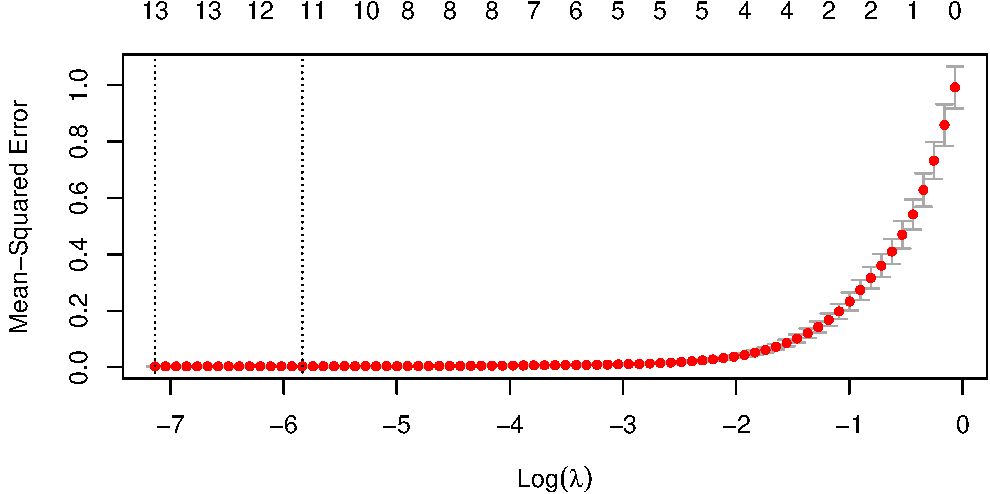
\includegraphics{Statistical_Learning_Final_Report_files/figure-latex/lasso_regression-1} \end{center}

\begin{Shaded}
\begin{Highlighting}[]
\NormalTok{lasso\_coef }\OtherTok{\textless{}{-}} \FunctionTok{coef}\NormalTok{(mod\_lasso, }\AttributeTok{s =} \StringTok{"lambda.min"}\NormalTok{)}
\NormalTok{lasso\_coef}
\end{Highlighting}
\end{Shaded}

\begin{verbatim}
## 15 x 1 sparse Matrix of class "dgCMatrix"
##                                s1
## (Intercept)          1.569504e-17
## Total_Fat            2.813714e-01
## Trans_Fat           -1.213127e-02
## Saturated_Fat        .           
## Sodium              -2.136716e-02
## Total_Carbohydrates  1.879088e-02
## Cholesterol          6.957617e-01
## Dietary_Fibre        2.340655e-02
## Sugars               9.354308e-02
## Protein              5.873156e-02
## Vitamin_A            1.006149e-02
## Vitamin_C            2.526001e-02
## Calcium              1.080519e-01
## Iron                -6.555492e-02
## Caffeine             6.612001e-03
\end{verbatim}

The lasso regression model selects the most important features in the
data and penalizes the coefficients of the model. The model has a low
AIC and BIC values, the R-squared value is 0.99 so the model is a good
fit for the data.

\subsection{Ridge Regression}\label{ridge-regression}

We use the glmnet package to fit a ridge regression model. Ridge
regression is a type of linear regression that uses L2 regularization to
penalize the coefficients of the model. This helps to prevent
overfitting and reduce the impact of collinearity in the data.

\begin{Shaded}
\begin{Highlighting}[]
\NormalTok{mod\_ridge }\OtherTok{\textless{}{-}} \FunctionTok{cv.glmnet}\NormalTok{(}\AttributeTok{x =} \FunctionTok{as.matrix}\NormalTok{(std\_data[, }\SpecialCharTok{{-}}\DecValTok{1}\NormalTok{]),}
                       \AttributeTok{y =}\NormalTok{ std\_data}\SpecialCharTok{$}\NormalTok{Calories,}
                       \AttributeTok{alpha =} \DecValTok{0}\NormalTok{, }\AttributeTok{standardize =} \ConstantTok{FALSE}\NormalTok{)}
\FunctionTok{plot}\NormalTok{(mod\_ridge)}
\end{Highlighting}
\end{Shaded}

\begin{center}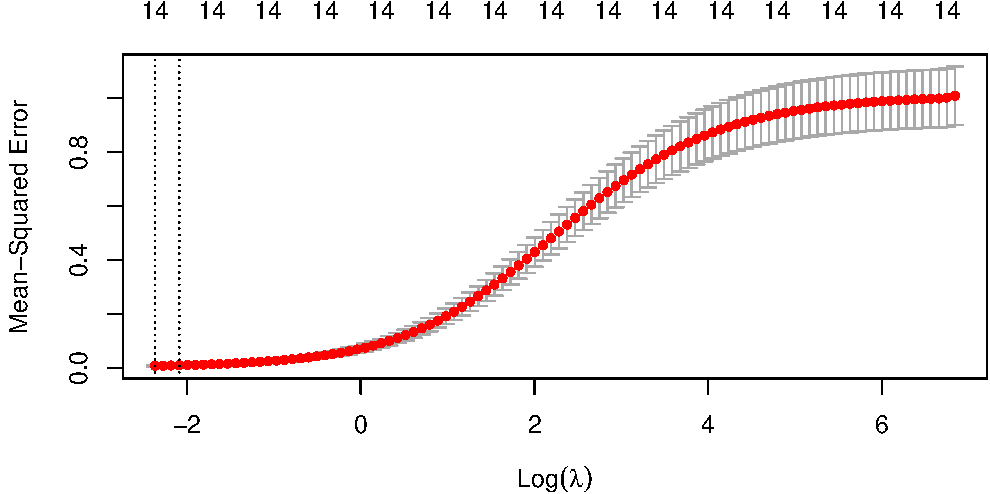
\includegraphics{Statistical_Learning_Final_Report_files/figure-latex/ridge_regression-1} \end{center}

\begin{Shaded}
\begin{Highlighting}[]
\NormalTok{ridge\_coef }\OtherTok{\textless{}{-}} \FunctionTok{coef}\NormalTok{(mod\_ridge, }\AttributeTok{s =} \StringTok{"lambda.min"}\NormalTok{)}
\NormalTok{ridge\_coef}
\end{Highlighting}
\end{Shaded}

\begin{verbatim}
## 15 x 1 sparse Matrix of class "dgCMatrix"
##                                s1
## (Intercept)          2.767416e-17
## Total_Fat            1.790461e-01
## Trans_Fat            5.621285e-02
## Saturated_Fat        9.206930e-03
## Sodium              -1.003136e-02
## Total_Carbohydrates  6.670660e-02
## Cholesterol          3.488854e-01
## Dietary_Fibre        5.575676e-02
## Sugars               3.437989e-01
## Protein              6.986559e-02
## Vitamin_A            5.069011e-03
## Vitamin_C            3.983592e-02
## Calcium              1.076895e-01
## Iron                -1.329709e-02
## Caffeine             1.007714e-04
\end{verbatim}

The ridge regression model reduces the impact of collinearity in the
data and penalizes the coefficients of the model. The model has a low
AIC and BIC values, the R-squared value is 0.99 so the model is a good
fit for the data.

\subsection{Model Comparison}\label{model-comparison}

We compare the linear regression, lasso regression, and ridge regression
models to select the best model for predicting the amount of calories
based on the amount of the other variables. We evaluate the models using
the R-squared value, and the Mean Squared Error (MSE) for each model.

The R-squared value is a measure of how well the model fits the data, it
ranges from 0 to 1, with higher values indicating a better fit

\begin{Shaded}
\begin{Highlighting}[]
\NormalTok{lasso\_pred }\OtherTok{\textless{}{-}} \FunctionTok{predict}\NormalTok{(mod\_lasso, }\AttributeTok{s =} \StringTok{"lambda.min"}\NormalTok{, }
                      \AttributeTok{newx =} \FunctionTok{as.matrix}\NormalTok{(std\_data[, }\SpecialCharTok{{-}}\DecValTok{1}\NormalTok{]))}
\NormalTok{lasso\_r\_squared }\OtherTok{\textless{}{-}} \FunctionTok{cor}\NormalTok{(lasso\_pred, std\_data}\SpecialCharTok{$}\NormalTok{Calories)}\SpecialCharTok{\^{}}\DecValTok{2}
\NormalTok{ridge\_pred }\OtherTok{\textless{}{-}} \FunctionTok{predict}\NormalTok{(mod\_ridge, }\AttributeTok{s =} \StringTok{"lambda.min"}\NormalTok{, }
                      \AttributeTok{newx =} \FunctionTok{as.matrix}\NormalTok{(std\_data[, }\SpecialCharTok{{-}}\DecValTok{1}\NormalTok{]))}
\NormalTok{ridge\_r\_squared }\OtherTok{\textless{}{-}} \FunctionTok{cor}\NormalTok{(ridge\_pred, std\_data}\SpecialCharTok{$}\NormalTok{Calories)}\SpecialCharTok{\^{}}\DecValTok{2}

\FunctionTok{kable}\NormalTok{(}\FunctionTok{data.frame}\NormalTok{(}\AttributeTok{Model =} \FunctionTok{c}\NormalTok{(}\StringTok{"Linear Regression"}\NormalTok{, }\StringTok{"Lasso Regression"}\NormalTok{,}
                           \StringTok{"Ridge Regression"}\NormalTok{),}
                 \AttributeTok{R\_squared =} \FunctionTok{c}\NormalTok{(}\FunctionTok{summary}\NormalTok{(lm\_model)}\SpecialCharTok{$}\NormalTok{r.squared,}
\NormalTok{                               lasso\_r\_squared, ridge\_r\_squared)), }
      \AttributeTok{caption =} \StringTok{"R{-}squared values for the models"}\NormalTok{)}
\end{Highlighting}
\end{Shaded}

\begin{longtable}[]{@{}lr@{}}
\caption{R-squared values for the models}\tabularnewline
\toprule\noalign{}
Model & R\_squared \\
\midrule\noalign{}
\endfirsthead
\toprule\noalign{}
Model & R\_squared \\
\midrule\noalign{}
\endhead
\bottomrule\noalign{}
\endlastfoot
Linear Regression & 0.9976608 \\
Lasso Regression & 0.9975756 \\
Ridge Regression & 0.9941815 \\
\end{longtable}

\subsection{Model Evaluation}\label{model-evaluation}

We evaluate the performance of the linear regression, lasso regression,
and ridge regression models using the mean squared error (MSE). The MSE
is a measure of the average squared difference between the predicted and
actual values. Lower values of the MSE indicate better performance of
the model.

\begin{Shaded}
\begin{Highlighting}[]
\NormalTok{linear\_pred }\OtherTok{\textless{}{-}} \FunctionTok{predict}\NormalTok{(lm\_model, }\AttributeTok{newdata =}\NormalTok{ data\_num)}
\NormalTok{linear\_mse }\OtherTok{\textless{}{-}} \FunctionTok{mean}\NormalTok{((linear\_pred }\SpecialCharTok{{-}}\NormalTok{ data\_num}\SpecialCharTok{$}\NormalTok{Calories)}\SpecialCharTok{\^{}}\DecValTok{2}\NormalTok{)}
\NormalTok{lasso\_mse }\OtherTok{\textless{}{-}} \FunctionTok{mean}\NormalTok{((lasso\_pred }\SpecialCharTok{{-}}\NormalTok{ std\_data}\SpecialCharTok{$}\NormalTok{Calories)}\SpecialCharTok{\^{}}\DecValTok{2}\NormalTok{)}
\NormalTok{ridge\_mse }\OtherTok{\textless{}{-}} \FunctionTok{mean}\NormalTok{((ridge\_pred }\SpecialCharTok{{-}}\NormalTok{ std\_data}\SpecialCharTok{$}\NormalTok{Calories)}\SpecialCharTok{\^{}}\DecValTok{2}\NormalTok{)}

\FunctionTok{kable}\NormalTok{(}\FunctionTok{data.frame}\NormalTok{(}\AttributeTok{Model =} \FunctionTok{c}\NormalTok{(}\StringTok{"Linear Regression"}\NormalTok{,}
                           \StringTok{"Lasso Regression"}\NormalTok{, }\StringTok{"Ridge Regression"}\NormalTok{),}
                 \AttributeTok{MSE =} \FunctionTok{c}\NormalTok{(linear\_mse, lasso\_mse, ridge\_mse)), }
      \AttributeTok{caption =} \StringTok{"MSE values for the models"}\NormalTok{)}
\end{Highlighting}
\end{Shaded}

\begin{longtable}[]{@{}lr@{}}
\caption{MSE values for the models}\tabularnewline
\toprule\noalign{}
Model & MSE \\
\midrule\noalign{}
\endfirsthead
\toprule\noalign{}
Model & MSE \\
\midrule\noalign{}
\endhead
\bottomrule\noalign{}
\endlastfoot
Linear Regression & 24.6481166 \\
Lasso Regression & 0.0024158 \\
Ridge Regression & 0.0066477 \\
\end{longtable}

We choose the model with the highest R-squared value and the lowest MSE
as the best model for predicting the amount of calories based on the
amount of the other variables. The best model is the lasso because it
has the lowest value for R\^{}2 and MSE and it is the most robust model.

\subsection{Cross Validation}\label{cross-validation}

Cross validation is a technique used to evaluate the performance of a
model. It involves splitting the data into training and testing sets,
fitting the model using the training set, and evaluating the model using
the testing set. This process is repeated multiple times to ensure that
the model is robust and generalizes well to new data.

We split the data into training and testing sets, fit the lasso
regression model using the training set.

\begin{Shaded}
\begin{Highlighting}[]
\FunctionTok{set.seed}\NormalTok{(}\DecValTok{123}\NormalTok{)}
\NormalTok{train\_index }\OtherTok{\textless{}{-}} \FunctionTok{sample}\NormalTok{(}\DecValTok{1}\SpecialCharTok{:}\FunctionTok{nrow}\NormalTok{(std\_data), }\FloatTok{0.8} \SpecialCharTok{*} \FunctionTok{nrow}\NormalTok{(std\_data))}
\NormalTok{train\_data }\OtherTok{\textless{}{-}}\NormalTok{ std\_data[train\_index, ]}
\NormalTok{test\_data }\OtherTok{\textless{}{-}}\NormalTok{ std\_data[}\SpecialCharTok{{-}}\NormalTok{train\_index, ]}
\CommentTok{\# Fit the lasso regression model on the training data}
\NormalTok{mod\_lasso\_train }\OtherTok{\textless{}{-}} \FunctionTok{cv.glmnet}\NormalTok{(}\AttributeTok{x =} \FunctionTok{as.matrix}\NormalTok{(train\_data[, }\SpecialCharTok{{-}}\DecValTok{1}\NormalTok{]),}
                             \AttributeTok{y =}\NormalTok{ train\_data}\SpecialCharTok{$}\NormalTok{Calories,}
                             \AttributeTok{alpha =} \DecValTok{1}\NormalTok{, }\AttributeTok{standardize =} \ConstantTok{FALSE}\NormalTok{)}
\end{Highlighting}
\end{Shaded}

We evaluate the model using the testing set. We make predictions using
the testing set and calculate the mean squared error and the root mean
squared error to assess the model's accuracy.

\begin{Shaded}
\begin{Highlighting}[]
\NormalTok{lasso\_pred\_test }\OtherTok{\textless{}{-}} \FunctionTok{predict}\NormalTok{(mod\_lasso\_train, }\AttributeTok{s =} \StringTok{"lambda.min"}\NormalTok{,}
                           \AttributeTok{newx =} \FunctionTok{as.matrix}\NormalTok{(test\_data[, }\SpecialCharTok{{-}}\DecValTok{1}\NormalTok{]))}
\CommentTok{\# R{-}squared value of the lasso regression model on the test data}
\NormalTok{lasso\_r\_squared\_test }\OtherTok{\textless{}{-}} \FunctionTok{cor}\NormalTok{(lasso\_pred\_test, test\_data}\SpecialCharTok{$}\NormalTok{Calories)}\SpecialCharTok{\^{}}\DecValTok{2}
\CommentTok{\# MSE of the lasso regression model on the test data}
\NormalTok{lasso\_mse\_test }\OtherTok{\textless{}{-}} \FunctionTok{mean}\NormalTok{((lasso\_pred\_test }\SpecialCharTok{{-}}\NormalTok{ test\_data}\SpecialCharTok{$}\NormalTok{Calories)}\SpecialCharTok{\^{}}\DecValTok{2}\NormalTok{)}
\end{Highlighting}
\end{Shaded}

The R-squared value and MSE are used to evaluate the performance of the
model on the test data.

\begin{Shaded}
\begin{Highlighting}[]
\CommentTok{\# Accuracy of the model}
\NormalTok{accuracy\_lm }\OtherTok{\textless{}{-}} \DecValTok{1} \SpecialCharTok{{-}}\NormalTok{ (lasso\_mse\_test }\SpecialCharTok{/} \FunctionTok{var}\NormalTok{(test\_data}\SpecialCharTok{$}\NormalTok{Calories))}
\CommentTok{\# Plot the predicted values against the actual values on the test data}
\FunctionTok{plot}\NormalTok{(test\_data}\SpecialCharTok{$}\NormalTok{Calories, lasso\_pred\_test, }\AttributeTok{xlab =} \StringTok{"Actual Calories"}\NormalTok{,}
     \AttributeTok{ylab =} \StringTok{"Predicted Calories"}\NormalTok{, }\AttributeTok{main =} \StringTok{"Predicted vs Actual Calories"}\NormalTok{,}
     \AttributeTok{col =} \StringTok{"\#4ea5ff"}\NormalTok{, }\AttributeTok{pch =} \DecValTok{19}\NormalTok{)}
\FunctionTok{abline}\NormalTok{(}\DecValTok{0}\NormalTok{, }\DecValTok{1}\NormalTok{, }\AttributeTok{col =} \StringTok{"\#ff810f"}\NormalTok{, }\AttributeTok{lwd =} \DecValTok{2}\NormalTok{)}
\end{Highlighting}
\end{Shaded}

\begin{center}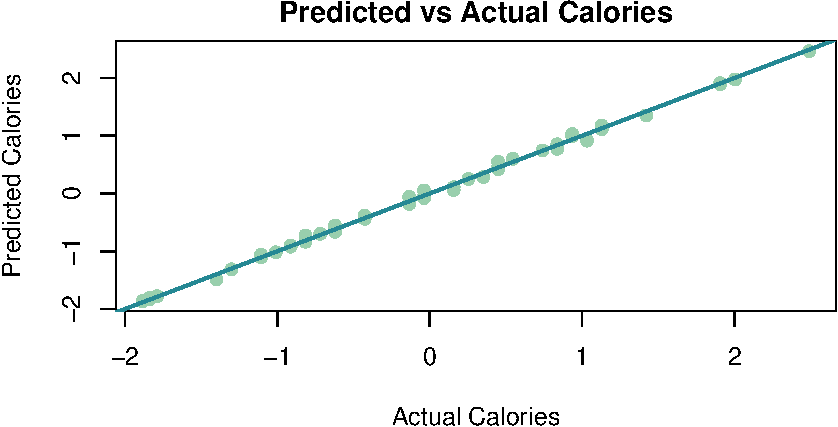
\includegraphics{Statistical_Learning_Final_Report_files/figure-latex/accuracy_lm-1} \end{center}

\begin{Shaded}
\begin{Highlighting}[]
\FunctionTok{kable}\NormalTok{(}\FunctionTok{data.frame}\NormalTok{(}\AttributeTok{Accuracy =}\NormalTok{ accuracy\_lm, }\AttributeTok{MSE =}\NormalTok{ lasso\_mse\_test, }
                 \AttributeTok{R\_squared =}\NormalTok{ lasso\_r\_squared\_test),}
      \AttributeTok{caption =} \StringTok{"Model evaluation metrics on the test data"}\NormalTok{)}
\end{Highlighting}
\end{Shaded}

\begin{longtable}[]{@{}lrrr@{}}
\caption{Model evaluation metrics on the test data}\tabularnewline
\toprule\noalign{}
& Accuracy & MSE & R\_squared \\
\midrule\noalign{}
\endfirsthead
\toprule\noalign{}
& Accuracy & MSE & R\_squared \\
\midrule\noalign{}
\endhead
\bottomrule\noalign{}
\endlastfoot
lambda.min & 0.9979473 & 0.0026283 & 0.9979454 \\
\end{longtable}

As we can see from \emph{Table 7} the R-squared value is 0.997,
indicating that the model explains 99\% of the variance in the data and
the MSE is 0.002628338, indicating that the model has a low error rate.
The accuracy of the model is 0.9979473, indicating that the model is
able to predict the amount of calories with high accuracy. The plot
shows the predicted values against the actual values on the test data
The points are close to the diagonal line, indicating that the model is
making accurate predictions.

\end{document}
